% Options for packages loaded elsewhere
\PassOptionsToPackage{unicode}{hyperref}
\PassOptionsToPackage{hyphens}{url}
%
\documentclass[
]{article}
\usepackage{amsmath,amssymb}
\usepackage{iftex}
\ifPDFTeX
  \usepackage[T1]{fontenc}
  \usepackage[utf8]{inputenc}
  \usepackage{textcomp} % provide euro and other symbols
\else % if luatex or xetex
  \usepackage{unicode-math} % this also loads fontspec
  \defaultfontfeatures{Scale=MatchLowercase}
  \defaultfontfeatures[\rmfamily]{Ligatures=TeX,Scale=1}
\fi
\usepackage{lmodern}
\ifPDFTeX\else
  % xetex/luatex font selection
\fi
% Use upquote if available, for straight quotes in verbatim environments
\IfFileExists{upquote.sty}{\usepackage{upquote}}{}
\IfFileExists{microtype.sty}{% use microtype if available
  \usepackage[]{microtype}
  \UseMicrotypeSet[protrusion]{basicmath} % disable protrusion for tt fonts
}{}
\makeatletter
\@ifundefined{KOMAClassName}{% if non-KOMA class
  \IfFileExists{parskip.sty}{%
    \usepackage{parskip}
  }{% else
    \setlength{\parindent}{0pt}
    \setlength{\parskip}{6pt plus 2pt minus 1pt}}
}{% if KOMA class
  \KOMAoptions{parskip=half}}
\makeatother
\usepackage{xcolor}
\usepackage[margin=1in]{geometry}
\usepackage{color}
\usepackage{fancyvrb}
\newcommand{\VerbBar}{|}
\newcommand{\VERB}{\Verb[commandchars=\\\{\}]}
\DefineVerbatimEnvironment{Highlighting}{Verbatim}{commandchars=\\\{\}}
% Add ',fontsize=\small' for more characters per line
\usepackage{framed}
\definecolor{shadecolor}{RGB}{248,248,248}
\newenvironment{Shaded}{\begin{snugshade}}{\end{snugshade}}
\newcommand{\AlertTok}[1]{\textcolor[rgb]{0.94,0.16,0.16}{#1}}
\newcommand{\AnnotationTok}[1]{\textcolor[rgb]{0.56,0.35,0.01}{\textbf{\textit{#1}}}}
\newcommand{\AttributeTok}[1]{\textcolor[rgb]{0.13,0.29,0.53}{#1}}
\newcommand{\BaseNTok}[1]{\textcolor[rgb]{0.00,0.00,0.81}{#1}}
\newcommand{\BuiltInTok}[1]{#1}
\newcommand{\CharTok}[1]{\textcolor[rgb]{0.31,0.60,0.02}{#1}}
\newcommand{\CommentTok}[1]{\textcolor[rgb]{0.56,0.35,0.01}{\textit{#1}}}
\newcommand{\CommentVarTok}[1]{\textcolor[rgb]{0.56,0.35,0.01}{\textbf{\textit{#1}}}}
\newcommand{\ConstantTok}[1]{\textcolor[rgb]{0.56,0.35,0.01}{#1}}
\newcommand{\ControlFlowTok}[1]{\textcolor[rgb]{0.13,0.29,0.53}{\textbf{#1}}}
\newcommand{\DataTypeTok}[1]{\textcolor[rgb]{0.13,0.29,0.53}{#1}}
\newcommand{\DecValTok}[1]{\textcolor[rgb]{0.00,0.00,0.81}{#1}}
\newcommand{\DocumentationTok}[1]{\textcolor[rgb]{0.56,0.35,0.01}{\textbf{\textit{#1}}}}
\newcommand{\ErrorTok}[1]{\textcolor[rgb]{0.64,0.00,0.00}{\textbf{#1}}}
\newcommand{\ExtensionTok}[1]{#1}
\newcommand{\FloatTok}[1]{\textcolor[rgb]{0.00,0.00,0.81}{#1}}
\newcommand{\FunctionTok}[1]{\textcolor[rgb]{0.13,0.29,0.53}{\textbf{#1}}}
\newcommand{\ImportTok}[1]{#1}
\newcommand{\InformationTok}[1]{\textcolor[rgb]{0.56,0.35,0.01}{\textbf{\textit{#1}}}}
\newcommand{\KeywordTok}[1]{\textcolor[rgb]{0.13,0.29,0.53}{\textbf{#1}}}
\newcommand{\NormalTok}[1]{#1}
\newcommand{\OperatorTok}[1]{\textcolor[rgb]{0.81,0.36,0.00}{\textbf{#1}}}
\newcommand{\OtherTok}[1]{\textcolor[rgb]{0.56,0.35,0.01}{#1}}
\newcommand{\PreprocessorTok}[1]{\textcolor[rgb]{0.56,0.35,0.01}{\textit{#1}}}
\newcommand{\RegionMarkerTok}[1]{#1}
\newcommand{\SpecialCharTok}[1]{\textcolor[rgb]{0.81,0.36,0.00}{\textbf{#1}}}
\newcommand{\SpecialStringTok}[1]{\textcolor[rgb]{0.31,0.60,0.02}{#1}}
\newcommand{\StringTok}[1]{\textcolor[rgb]{0.31,0.60,0.02}{#1}}
\newcommand{\VariableTok}[1]{\textcolor[rgb]{0.00,0.00,0.00}{#1}}
\newcommand{\VerbatimStringTok}[1]{\textcolor[rgb]{0.31,0.60,0.02}{#1}}
\newcommand{\WarningTok}[1]{\textcolor[rgb]{0.56,0.35,0.01}{\textbf{\textit{#1}}}}
\usepackage{graphicx}
\makeatletter
\def\maxwidth{\ifdim\Gin@nat@width>\linewidth\linewidth\else\Gin@nat@width\fi}
\def\maxheight{\ifdim\Gin@nat@height>\textheight\textheight\else\Gin@nat@height\fi}
\makeatother
% Scale images if necessary, so that they will not overflow the page
% margins by default, and it is still possible to overwrite the defaults
% using explicit options in \includegraphics[width, height, ...]{}
\setkeys{Gin}{width=\maxwidth,height=\maxheight,keepaspectratio}
% Set default figure placement to htbp
\makeatletter
\def\fps@figure{htbp}
\makeatother
\setlength{\emergencystretch}{3em} % prevent overfull lines
\providecommand{\tightlist}{%
  \setlength{\itemsep}{0pt}\setlength{\parskip}{0pt}}
\setcounter{secnumdepth}{-\maxdimen} % remove section numbering
\usepackage{mathrsfs}
\usepackage{amsfonts}
\ifLuaTeX
  \usepackage{selnolig}  % disable illegal ligatures
\fi
\IfFileExists{bookmark.sty}{\usepackage{bookmark}}{\usepackage{hyperref}}
\IfFileExists{xurl.sty}{\usepackage{xurl}}{} % add URL line breaks if available
\urlstyle{same}
\hypersetup{
  pdftitle={Problem Set 3 Longitudinal Bootstrap Code},
  hidelinks,
  pdfcreator={LaTeX via pandoc}}

\title{Problem Set 3 Longitudinal Bootstrap Code}
\author{}
\date{\vspace{-2.5em}}

\begin{document}
\maketitle

\begin{Shaded}
\begin{Highlighting}[]
\NormalTok{knitr}\SpecialCharTok{::}\NormalTok{opts\_chunk}\SpecialCharTok{$}\FunctionTok{set}\NormalTok{(}\AttributeTok{warning =} \ConstantTok{FALSE}\NormalTok{)}
\FunctionTok{library}\NormalTok{(nlme)}
\FunctionTok{library}\NormalTok{(tidyverse)}
\FunctionTok{library}\NormalTok{(gee)}
\FunctionTok{library}\NormalTok{(lmtest)}
\FunctionTok{library}\NormalTok{(splines)}
\FunctionTok{library}\NormalTok{(ggplot2)}
\FunctionTok{library}\NormalTok{(gridExtra)}
\FunctionTok{library}\NormalTok{(dplyr)}
\FunctionTok{library}\NormalTok{(boot)}

\FunctionTok{options}\NormalTok{(}\AttributeTok{digits =} \DecValTok{3}\NormalTok{)}
\end{Highlighting}
\end{Shaded}

\hypertarget{part-i-get-familiar-with-the-data}{%
\section{Part I: Get familiar with the
data}\label{part-i-get-familiar-with-the-data}}

\hypertarget{load-the-data-and-create-the-parity-variable}{%
\subsubsection{Load the data and create the parity
variable}\label{load-the-data-and-create-the-parity-variable}}

1.Read in the Nepal study data, keep only the necessary variables,
create the weight-for-age z-scores and indicator for female sex and
exclude visits with missing weight-for-age z-scores or where children
are over 60 months of age.

\begin{Shaded}
\begin{Highlighting}[]
\FunctionTok{load}\NormalTok{(}\StringTok{"nepal.anthro.rdata"}\NormalTok{)}
\NormalTok{d0 }\OtherTok{=}\NormalTok{ nepal.anthro[,}\FunctionTok{c}\NormalTok{(}\StringTok{"id"}\NormalTok{, }\StringTok{"alive"}\NormalTok{, }\StringTok{"age"}\NormalTok{, }\StringTok{"wt"}\NormalTok{,}\StringTok{"fuvisit"}\NormalTok{,}\StringTok{"sex"}\NormalTok{)]}
\NormalTok{d0}\SpecialCharTok{$}\NormalTok{female }\OtherTok{=} \FunctionTok{factor}\NormalTok{(}\FunctionTok{ifelse}\NormalTok{(d0}\SpecialCharTok{$}\NormalTok{sex}\SpecialCharTok{==}\DecValTok{2}\NormalTok{,}\DecValTok{1}\NormalTok{,}\DecValTok{0}\NormalTok{),}\AttributeTok{levels=}\DecValTok{0}\SpecialCharTok{:}\DecValTok{1}\NormalTok{,}\AttributeTok{labels=}\FunctionTok{c}\NormalTok{(}\StringTok{"Male"}\NormalTok{,}\StringTok{"Female"}\NormalTok{))}
\CommentTok{\# install.packages("anthro")}
\FunctionTok{library}\NormalTok{(anthro)}
\NormalTok{zscores }\OtherTok{=} \FunctionTok{with}\NormalTok{(d0,}\FunctionTok{anthro\_zscores}\NormalTok{(}\AttributeTok{sex =}\NormalTok{ sex, }\AttributeTok{age =}\NormalTok{ age,}\AttributeTok{weight =}\NormalTok{ wt,}\AttributeTok{is\_age\_in\_month=}\ConstantTok{TRUE}\NormalTok{))}\SpecialCharTok{$}\NormalTok{zwei}
\NormalTok{d }\OtherTok{=} \FunctionTok{cbind}\NormalTok{(d0,zscores)[}\FunctionTok{complete.cases}\NormalTok{(d0) }\SpecialCharTok{\&}\NormalTok{ d0}\SpecialCharTok{$}\NormalTok{age}\SpecialCharTok{\textless{}=}\DecValTok{60}\NormalTok{,]}
\NormalTok{d\_clean }\OtherTok{\textless{}{-}}\NormalTok{ d }\SpecialCharTok{|\textgreater{}}
   \FunctionTok{filter}\NormalTok{(}\SpecialCharTok{!}\FunctionTok{is.na}\NormalTok{(zscores) }\SpecialCharTok{|}\NormalTok{ zscores }\SpecialCharTok{!=} \StringTok{\textquotesingle{}\textquotesingle{}}\NormalTok{ )}

\FunctionTok{summary}\NormalTok{(d\_clean}\SpecialCharTok{$}\NormalTok{zscores)}
\end{Highlighting}
\end{Shaded}

\begin{verbatim}
##    Min. 1st Qu.  Median    Mean 3rd Qu.    Max. 
##   -6.12   -2.54   -1.88   -1.97   -1.27    0.71
\end{verbatim}

\hypertarget{identify-the-number-of-children-in-the-sample-overall-and-for-each-sex.}{%
\subsubsection{2.Identify the number of children in the sample, overall
and for each
sex.}\label{identify-the-number-of-children-in-the-sample-overall-and-for-each-sex.}}

\begin{Shaded}
\begin{Highlighting}[]
\CommentTok{\# number of children in the sample}
\FunctionTok{n\_distinct}\NormalTok{(d\_clean}\SpecialCharTok{$}\NormalTok{id)    }\CommentTok{\#1: How many distinct participants? 195}
\end{Highlighting}
\end{Shaded}

\begin{verbatim}
## [1] 195
\end{verbatim}

\begin{Shaded}
\begin{Highlighting}[]
\CommentTok{\# Number of children by sex}
\NormalTok{n\_child\_sex }\OtherTok{=}\NormalTok{ d\_clean }\SpecialCharTok{\%\textgreater{}\%}
 \FunctionTok{group\_by}\NormalTok{(female) }\SpecialCharTok{\%\textgreater{}\%}
 \FunctionTok{summarise}\NormalTok{(}\AttributeTok{num\_children =} \FunctionTok{n\_distinct}\NormalTok{(id))}

\NormalTok{n\_child\_sex}
\end{Highlighting}
\end{Shaded}

\begin{verbatim}
## # A tibble: 2 x 2
##   female num_children
##   <fct>         <int>
## 1 Male            102
## 2 Female           93
\end{verbatim}

\hypertarget{calculate-the-number-of-visits-for-each-child-with-non-missing-weight-for-age-z-scores-and-compute-the-average-and-quartiles-of-the-number-of-visits-for-each-child-by-sex.}{%
\paragraph{Calculate the number of visits for each child with
non-missing weight-for-age z-scores and compute the average and
quartiles of the number of visits for each child by
sex.}\label{calculate-the-number-of-visits-for-each-child-with-non-missing-weight-for-age-z-scores-and-compute-the-average-and-quartiles-of-the-number-of-visits-for-each-child-by-sex.}}

\begin{Shaded}
\begin{Highlighting}[]
\CommentTok{\# number of visits for each child with non{-}missing z{-}scores }
\NormalTok{visits\_per\_child }\OtherTok{\textless{}{-}} \FunctionTok{aggregate}\NormalTok{(zscores }\SpecialCharTok{\textasciitilde{}}\NormalTok{ id, }\AttributeTok{data=}\NormalTok{d\_clean, }\ControlFlowTok{function}\NormalTok{(x) }\FunctionTok{sum}\NormalTok{(}\SpecialCharTok{!}\FunctionTok{is.na}\NormalTok{(x)))}
\FunctionTok{names}\NormalTok{(visits\_per\_child) }\OtherTok{\textless{}{-}} \FunctionTok{c}\NormalTok{(}\StringTok{"id"}\NormalTok{, }\StringTok{"num\_visits"}\NormalTok{)}
\NormalTok{visits\_per\_child}
\end{Highlighting}
\end{Shaded}

\begin{verbatim}
##         id num_visits
## 1   120011          4
## 2   120012          1
## 3   120021          5
## 4   120022          4
## 5   120023          3
## 6   120031          3
## 7   120051          5
## 8   120052          5
## 9   120053          2
## 10  120061          5
## 11  120062          1
## 12  120071          5
## 13  120072          2
## 14  120081          5
## 15  120082          5
## 16  120091          5
## 17  120111          3
## 18  120112          2
## 19  120121          4
## 20  120131          5
## 21  120132          5
## 22  120133          2
## 23  120141          5
## 24  120142          2
## 25  120151          5
## 26  120152          5
## 27  120161          5
## 28  120162          5
## 29  120191          5
## 30  120192          4
## 31  120211          4
## 32  120212          5
## 33  120231          5
## 34  120241          1
## 35  120242          1
## 36  120251          5
## 37  120252          3
## 38  120261          5
## 39  120271          4
## 40  120291          4
## 41  120292          2
## 42  120321          5
## 43  120322          3
## 44  120331          2
## 45  120341          5
## 46  120342          3
## 47  120351          5
## 48  120352          5
## 49  120361          5
## 50  120362          5
## 51  120371          5
## 52  120372          5
## 53  120381          5
## 54  120382          2
## 55  120383          5
## 56  120384          4
## 57  120391          5
## 58  120392          5
## 59  120401          5
## 60  120402          5
## 61  120411          3
## 62  120412          3
## 63  120431          5
## 64  120441          5
## 65  120442          1
## 66  120443          3
## 67  120444          4
## 68  120451          5
## 69  120452          5
## 70  120453          1
## 71  120471          5
## 72  120472          5
## 73  120473          1
## 74  120541          5
## 75  120561          5
## 76  120571          5
## 77  120572          5
## 78  120581          5
## 79  120582          5
## 80  120591          5
## 81  120601          5
## 82  120602          5
## 83  120603          5
## 84  120611          5
## 85  120631          5
## 86  120632          1
## 87  120651          5
## 88  120671          5
## 89  120672          4
## 90  120681          5
## 91  120682          5
## 92  120683          4
## 93  120691          1
## 94  120692          5
## 95  360011          3
## 96  360012          3
## 97  360021          4
## 98  360051          5
## 99  360052          3
## 100 360111          1
## 101 360112          1
## 102 360113          3
## 103 360114          1
## 104 360121          4
## 105 360131          2
## 106 360132          2
## 107 360141          4
## 108 360161          3
## 109 360181          5
## 110 360191          5
## 111 360211          5
## 112 360221          5
## 113 360222          1
## 114 360223          3
## 115 360251          5
## 116 360301          5
## 117 360302          1
## 118 360331          4
## 119 360341          5
## 120 360351          5
## 121 360352          2
## 122 360353          3
## 123 360361          4
## 124 360362          3
## 125 360371          5
## 126 360372          3
## 127 360391          5
## 128 360392          2
## 129 360393          1
## 130 360411          5
## 131 360471          5
## 132 360472          5
## 133 360481          5
## 134 360482          5
## 135 360491          2
## 136 360501          5
## 137 360502          2
## 138 360511          4
## 139 360531          5
## 140 360541          4
## 141 360551          4
## 142 360561          5
## 143 360562          5
## 144 360571          3
## 145 360581          5
## 146 360591          5
## 147 360592          2
## 148 360611          5
## 149 360621          5
## 150 360671          1
## 151 360672          4
## 152 360673          5
## 153 360674          1
## 154 360691          5
## 155 360701          4
## 156 360711          1
## 157 360721          1
## 158 360741          5
## 159 360751          5
## 160 360752          1
## 161 360781          5
## 162 360782          2
## 163 360791          2
## 164 360801          5
## 165 360811          3
## 166 360812          3
## 167 360813          4
## 168 360841          4
## 169 360842          4
## 170 360871          5
## 171 360881          2
## 172 360901          2
## 173 360911          3
## 174 360912          3
## 175 360921          2
## 176 360941          5
## 177 360951          5
## 178 360952          2
## 179 360991          4
## 180 360992          5
## 181 361001          5
## 182 361002          1
## 183 520021          4
## 184 520022          3
## 185 520031          5
## 186 520041          5
## 187 520042          5
## 188 520051          3
## 189 520061          2
## 190 520062          3
## 191 520063          5
## 192 520071          4
## 193 520072          3
## 194 520081          5
## 195 520091          4
\end{verbatim}

\hypertarget{compute-average-and-quartiles-of-the-number-of-visits-for-each-child-by-sex}{%
\section{Compute Average and Quartiles of the Number of Visits for Each
Child by
Sex:}\label{compute-average-and-quartiles-of-the-number-of-visits-for-each-child-by-sex}}

\begin{Shaded}
\begin{Highlighting}[]
\CommentTok{\# Calculate the number of visits for each child with non{-}missing z{-}scores}
\NormalTok{visits\_per\_child\_sex }\OtherTok{\textless{}{-}} \FunctionTok{aggregate}\NormalTok{(fuvisit }\SpecialCharTok{\textasciitilde{}}\NormalTok{ id }\SpecialCharTok{+}\NormalTok{ sex, }\AttributeTok{data=}\NormalTok{d\_clean, }\AttributeTok{FUN=}\NormalTok{length)}

\CommentTok{\# Calculate the average number of visits by sex}
\NormalTok{average\_visits\_by\_sex }\OtherTok{\textless{}{-}} \FunctionTok{aggregate}\NormalTok{(fuvisit }\SpecialCharTok{\textasciitilde{}}\NormalTok{ sex, }\AttributeTok{data=}\NormalTok{visits\_per\_child\_sex, }\AttributeTok{FUN=}\NormalTok{mean)}

\CommentTok{\# Calculate the quartiles of the number of visits by sex}
\NormalTok{quartiles\_visits\_by\_sex }\OtherTok{\textless{}{-}} \FunctionTok{aggregate}\NormalTok{(fuvisit }\SpecialCharTok{\textasciitilde{}}\NormalTok{ sex, }\AttributeTok{data=}\NormalTok{visits\_per\_child\_sex, }\AttributeTok{FUN=}\ControlFlowTok{function}\NormalTok{(x) }\FunctionTok{quantile}\NormalTok{(x, }\AttributeTok{probs=}\FunctionTok{c}\NormalTok{(}\FloatTok{0.25}\NormalTok{, }\FloatTok{0.5}\NormalTok{, }\FloatTok{0.75}\NormalTok{)))}

\FunctionTok{colnames}\NormalTok{(average\_visits\_by\_sex) }\OtherTok{\textless{}{-}} \FunctionTok{c}\NormalTok{(}\StringTok{"Sex"}\NormalTok{, }\StringTok{"Average Visits"}\NormalTok{)}
\FunctionTok{colnames}\NormalTok{(quartiles\_visits\_by\_sex) }\OtherTok{\textless{}{-}} \FunctionTok{c}\NormalTok{(}\StringTok{"Sex"}\NormalTok{, }\StringTok{"Quartiles of Visits"}\NormalTok{)}

\FunctionTok{print}\NormalTok{(average\_visits\_by\_sex)}
\end{Highlighting}
\end{Shaded}

\begin{verbatim}
##   Sex Average Visits
## 1   1           3.76
## 2   2           3.86
\end{verbatim}

\begin{Shaded}
\begin{Highlighting}[]
\FunctionTok{print}\NormalTok{(quartiles\_visits\_by\_sex)}
\end{Highlighting}
\end{Shaded}

\begin{verbatim}
##   Sex Quartiles of Visits.25% Quartiles of Visits.50% Quartiles of Visits.75%
## 1   1                       3                       4                       5
## 2   2                       3                       5                       5
\end{verbatim}

The average of the number of visits is 3.86 for female, and 3.76 for
male.

\hypertarget{make-a-spaghetti-plot-of-childrens-weight-for-age-z-scores-as-a-function-of-age-connecting-the-measured-weights-within-a-child-over-time.-color-code-the-data-by-sex.-add-smoothing-splines-for-each-sex.-note-any-similarities-or-differences-in-the-growth-rates-across-the-groups.}{%
\subsubsection{3.Make a spaghetti plot of children's weight-for-age
z-scores as a function of age; connecting the measured weights within a
child over time. Color code the data by sex. Add smoothing splines for
each sex. Note any similarities or differences in the growth rates
across the
groups.}\label{make-a-spaghetti-plot-of-childrens-weight-for-age-z-scores-as-a-function-of-age-connecting-the-measured-weights-within-a-child-over-time.-color-code-the-data-by-sex.-add-smoothing-splines-for-each-sex.-note-any-similarities-or-differences-in-the-growth-rates-across-the-groups.}}

\begin{Shaded}
\begin{Highlighting}[]
\CommentTok{\# Create custom theme}
\NormalTok{custom\_theme }\OtherTok{\textless{}{-}} \FunctionTok{theme}\NormalTok{(}
  \AttributeTok{panel.background =} \FunctionTok{element\_blank}\NormalTok{(),}
  \AttributeTok{axis.ticks =} \FunctionTok{element\_blank}\NormalTok{(),}
  \AttributeTok{axis.text =} \FunctionTok{element\_text}\NormalTok{(}\AttributeTok{size =} \DecValTok{12}\NormalTok{),}
  \AttributeTok{axis.title =} \FunctionTok{element\_text}\NormalTok{(}\AttributeTok{size =} \DecValTok{12}\NormalTok{, }\AttributeTok{face =} \StringTok{"bold"}\NormalTok{),}
  \AttributeTok{axis.line =} \FunctionTok{element\_line}\NormalTok{(}\AttributeTok{size =} \FloatTok{0.5}\NormalTok{),}
  \AttributeTok{plot.title =} \FunctionTok{element\_text}\NormalTok{(}\AttributeTok{size =} \DecValTok{14}\NormalTok{, }\AttributeTok{face =} \StringTok{"bold"}\NormalTok{, }\AttributeTok{hjust =} \FloatTok{0.5}\NormalTok{)}
\NormalTok{)}

\CommentTok{\# Spaghetti plot of whole mouth average gingival index}
\NormalTok{spagplot }\OtherTok{\textless{}{-}}\NormalTok{ d\_clean }\SpecialCharTok{|\textgreater{}}
  \FunctionTok{ggplot}\NormalTok{() }\SpecialCharTok{+}
  \FunctionTok{geom\_line}\NormalTok{(}\FunctionTok{aes}\NormalTok{(}\AttributeTok{x =}\NormalTok{ age, }\AttributeTok{y =}\NormalTok{ zscores, }\AttributeTok{group =} \FunctionTok{factor}\NormalTok{(id), }\AttributeTok{color =}\NormalTok{ female), }\AttributeTok{linewidth =} \DecValTok{1}\NormalTok{, }\AttributeTok{alpha =} \FloatTok{0.5}\NormalTok{) }\SpecialCharTok{+}
  \FunctionTok{geom\_smooth}\NormalTok{(}\FunctionTok{aes}\NormalTok{(}\AttributeTok{x =}\NormalTok{ age, }\AttributeTok{y =}\NormalTok{ zscores, }\AttributeTok{color =}\NormalTok{ female), }\AttributeTok{method =} \StringTok{"loess"}\NormalTok{, }\AttributeTok{se =} \ConstantTok{FALSE}\NormalTok{) }\SpecialCharTok{+}
  \CommentTok{\# scale\_x\_discrete(labels = c("Baseline (1)", "3", "5")) +}
  \FunctionTok{labs}\NormalTok{(}\AttributeTok{x =} \StringTok{"Age (Months)"}\NormalTok{, }\AttributeTok{y =} \StringTok{"Weight{-}for{-}age z{-}scores"}\NormalTok{) }\SpecialCharTok{+}
  \FunctionTok{scale\_x\_continuous}\NormalTok{(}\AttributeTok{breaks =} \FunctionTok{seq}\NormalTok{(}\DecValTok{0}\NormalTok{,}\DecValTok{60}\NormalTok{,}\DecValTok{10}\NormalTok{),}\AttributeTok{limits =} \FunctionTok{c}\NormalTok{(}\DecValTok{0}\NormalTok{,}\DecValTok{60}\NormalTok{)) }\SpecialCharTok{+}
\NormalTok{  custom\_theme}
\NormalTok{spagplot}
\end{Highlighting}
\end{Shaded}

\begin{verbatim}
## `geom_smooth()` using formula = 'y ~ x'
\end{verbatim}

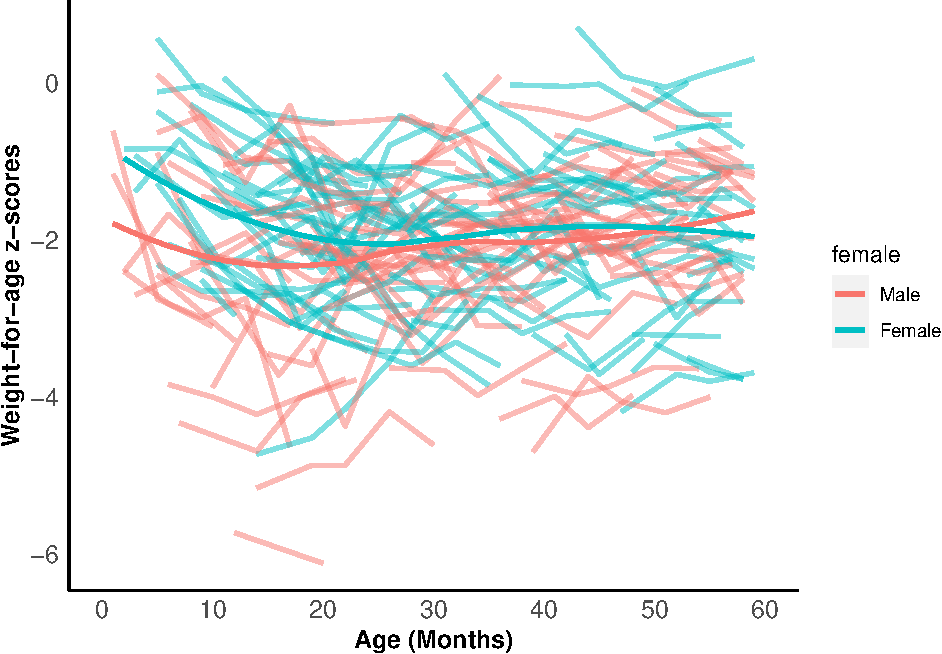
\includegraphics{ProblemSet3_ts_1677791812_files/figure-latex/unnamed-chunk-5-1.pdf}

\begin{Shaded}
\begin{Highlighting}[]
\NormalTok{spagplot\_mean }\OtherTok{\textless{}{-}}\NormalTok{ spagplot }\SpecialCharTok{+} 
  \FunctionTok{stat\_summary}\NormalTok{(}\AttributeTok{data =}\NormalTok{ d\_clean, }
               \AttributeTok{fun =}\NormalTok{ mean, }
               \AttributeTok{geom =} \StringTok{"line"}\NormalTok{,}
               \FunctionTok{aes}\NormalTok{(}\AttributeTok{x =}\NormalTok{ age, }\AttributeTok{y =}\NormalTok{ zscores, }\AttributeTok{group =}\NormalTok{ female, }\AttributeTok{color =}\NormalTok{ female), }
               \AttributeTok{linewidth =} \DecValTok{2}\NormalTok{) }
  \CommentTok{\# scale\_color\_manual(values = c("\#024873", "\#920043"),}
  \CommentTok{\#                    labels = c("Female", "Male"))}
\NormalTok{spagplot\_mean}
\end{Highlighting}
\end{Shaded}

\begin{verbatim}
## `geom_smooth()` using formula = 'y ~ x'
\end{verbatim}

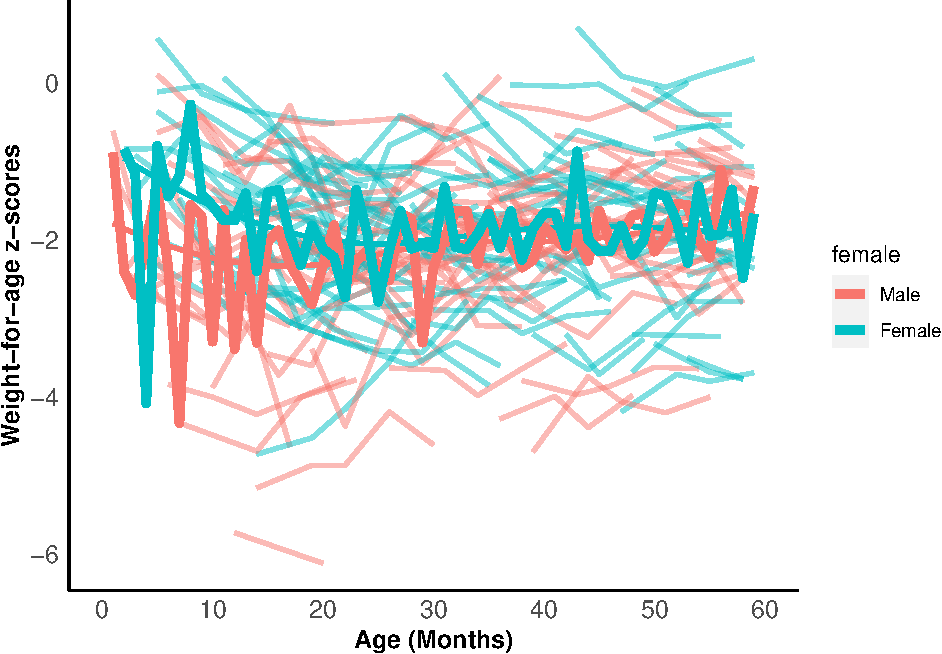
\includegraphics{ProblemSet3_ts_1677791812_files/figure-latex/unnamed-chunk-6-1.pdf}

We could see a increase trend in weight-for-age z-scores as age
increases in male. We could see a decreasing and then increasing trend
of weight-for-age z-scores as age increases in female

\hypertarget{part-ii-model-checking-and-recommendations}{%
\section{Part II: Model checking and
recommendations}\label{part-ii-model-checking-and-recommendations}}

\begin{Shaded}
\begin{Highlighting}[]
\NormalTok{model1 }\OtherTok{\textless{}{-}} \FunctionTok{lm}\NormalTok{(zscores }\SpecialCharTok{\textasciitilde{}}\NormalTok{ age }\SpecialCharTok{+}\NormalTok{ female }\SpecialCharTok{+}\NormalTok{ age}\SpecialCharTok{*}\NormalTok{female, }\AttributeTok{data =}\NormalTok{ d\_clean )}
\FunctionTok{summary}\NormalTok{(model1)}
\end{Highlighting}
\end{Shaded}

\begin{verbatim}
## 
## Call:
## lm(formula = zscores ~ age + female + age * female, data = d_clean)
## 
## Residuals:
##    Min     1Q Median     3Q    Max 
## -3.909 -0.580  0.084  0.656  2.615 
## 
## Coefficients:
##                  Estimate Std. Error t value Pr(>|t|)    
## (Intercept)      -2.43506    0.12361  -19.70  < 2e-16 ***
## age               0.01121    0.00338    3.32  0.00094 ***
## femaleFemale      0.69323    0.17316    4.00  6.9e-05 ***
## age:femaleFemale -0.01501    0.00476   -3.15  0.00170 ** 
## ---
## Signif. codes:  0 '***' 0.001 '**' 0.01 '*' 0.05 '.' 0.1 ' ' 1
## 
## Residual standard error: 0.993 on 739 degrees of freedom
## Multiple R-squared:  0.0257, Adjusted R-squared:  0.0217 
## F-statistic:  6.5 on 3 and 739 DF,  p-value: 0.000243
\end{verbatim}

\hypertarget{conduct-appropriate-checking-of-this-model-i.e.-check-for-appropriateness-of-the-mean-model-and-the-independence-and-constant-variance-assumptions-for-the-residuals.}{%
\subsubsection{1.Conduct appropriate checking of this model; i.e.~check
for appropriateness of the mean model, and the independence and constant
variance assumptions for the
residuals.}\label{conduct-appropriate-checking-of-this-model-i.e.-check-for-appropriateness-of-the-mean-model-and-the-independence-and-constant-variance-assumptions-for-the-residuals.}}

\hypertarget{assumption-ey-x-x-beta}{%
\paragraph{\texorpdfstring{assumption E(Y \textbar X) = X
\(\beta\)}{assumption E(Y \textbar X) = X \textbackslash beta}}\label{assumption-ey-x-x-beta}}

\begin{Shaded}
\begin{Highlighting}[]
\NormalTok{d\_clean}\SpecialCharTok{$}\NormalTok{residuals }\OtherTok{=} \FunctionTok{residuals}\NormalTok{(model1)}
\FunctionTok{ggplot}\NormalTok{(d\_clean,}\FunctionTok{aes}\NormalTok{(}\AttributeTok{x=}\NormalTok{age, }\AttributeTok{y=}\NormalTok{residuals)) }\SpecialCharTok{+}
    \FunctionTok{geom\_jitter}\NormalTok{(}\AttributeTok{alpha =} \FloatTok{0.7}\NormalTok{) }\SpecialCharTok{+}
    \FunctionTok{theme\_bw}\NormalTok{() }\SpecialCharTok{+}
    \FunctionTok{geom\_smooth}\NormalTok{() }\SpecialCharTok{+}
    \FunctionTok{geom\_hline}\NormalTok{(}\AttributeTok{yintercept=}\DecValTok{0}\NormalTok{,}\AttributeTok{color=}\StringTok{"red"}\NormalTok{) }\SpecialCharTok{+}
    \FunctionTok{labs}\NormalTok{(}\AttributeTok{y=}\StringTok{"Residuals: linear age"}\NormalTok{,}\AttributeTok{x=}\StringTok{"Age in months"}\NormalTok{) }\SpecialCharTok{+}
    \FunctionTok{scale\_y\_continuous}\NormalTok{(}\AttributeTok{breaks=}\FunctionTok{seq}\NormalTok{(}\SpecialCharTok{{-}}\FloatTok{3.5}\NormalTok{,}\FloatTok{3.5}\NormalTok{,}\FloatTok{0.5}\NormalTok{),}\AttributeTok{limits=}\FunctionTok{c}\NormalTok{(}\SpecialCharTok{{-}}\FloatTok{3.5}\NormalTok{,}\FloatTok{3.5}\NormalTok{)) }\SpecialCharTok{+}
  \FunctionTok{scale\_x\_continuous}\NormalTok{(}\AttributeTok{breaks=}\FunctionTok{seq}\NormalTok{(}\DecValTok{0}\NormalTok{,}\DecValTok{60}\NormalTok{,}\DecValTok{6}\NormalTok{),}\AttributeTok{limits=}\FunctionTok{c}\NormalTok{(}\DecValTok{0}\NormalTok{,}\DecValTok{60}\NormalTok{))}
\end{Highlighting}
\end{Shaded}

\begin{verbatim}
## `geom_smooth()` using method = 'loess' and formula = 'y ~ x'
\end{verbatim}

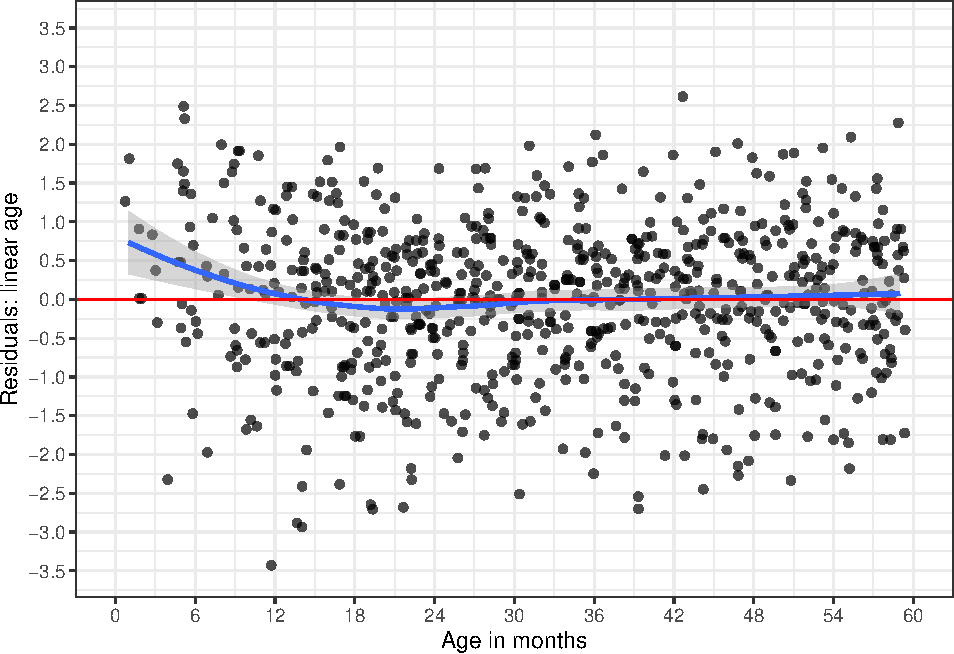
\includegraphics{ProblemSet3_ts_1677791812_files/figure-latex/unnamed-chunk-8-1.pdf}

\hypertarget{independence-assumption}{%
\paragraph{Independence assumption}\label{independence-assumption}}

Visualizing autocorrelation using a scatterplot matrix

\begin{Shaded}
\begin{Highlighting}[]
\CommentTok{\# Retrieve only the zscores, age, and Model 1}
\NormalTok{d\_wide }\OtherTok{\textless{}{-}}\NormalTok{ d\_clean }\SpecialCharTok{|\textgreater{}}
  \FunctionTok{select}\NormalTok{(residuals, fuvisit, id) }\SpecialCharTok{|\textgreater{}}
  \FunctionTok{pivot\_wider}\NormalTok{(}\AttributeTok{id\_cols =} \StringTok{"id"}\NormalTok{,}
              \AttributeTok{names\_from =} \StringTok{"fuvisit"}\NormalTok{,}
              \AttributeTok{values\_from =} \StringTok{"residuals"}\NormalTok{)}

\NormalTok{d\_wide }\OtherTok{\textless{}{-}}\NormalTok{ d\_wide }\SpecialCharTok{|\textgreater{}}
  \FunctionTok{filter}\NormalTok{(}\FunctionTok{complete.cases}\NormalTok{(d\_wide))}

\CommentTok{\# View the wide data}
\FunctionTok{head}\NormalTok{(d\_wide, }\AttributeTok{n =} \DecValTok{3}\NormalTok{)}
\end{Highlighting}
\end{Shaded}

\begin{verbatim}
## # A tibble: 3 x 6
##       id   `0`   `1`   `2`   `3`   `4`
##    <int> <dbl> <dbl> <dbl> <dbl> <dbl>
## 1 120021  1.50 1.17  0.903 0.608 0.523
## 2 120051  2.00 1.15  1.52  1.35  0.456
## 3 120052  1.03 0.608 0.554 0.709 0.514
\end{verbatim}

\begin{Shaded}
\begin{Highlighting}[]
\CommentTok{\# Use wide format of the data}
\FunctionTok{cor}\NormalTok{(d\_wide[,}\FunctionTok{c}\NormalTok{(}\DecValTok{2}\SpecialCharTok{:}\DecValTok{6}\NormalTok{)])}
\end{Highlighting}
\end{Shaded}

\begin{verbatim}
##       0     1     2     3     4
## 0 1.000 0.904 0.883 0.836 0.658
## 1 0.904 1.000 0.920 0.873 0.740
## 2 0.883 0.920 1.000 0.927 0.822
## 3 0.836 0.873 0.927 1.000 0.890
## 4 0.658 0.740 0.822 0.890 1.000
\end{verbatim}

\begin{Shaded}
\begin{Highlighting}[]
\FunctionTok{pairs}\NormalTok{(d\_wide[,}\FunctionTok{c}\NormalTok{(}\DecValTok{2}\SpecialCharTok{:}\DecValTok{6}\NormalTok{)])}
\end{Highlighting}
\end{Shaded}

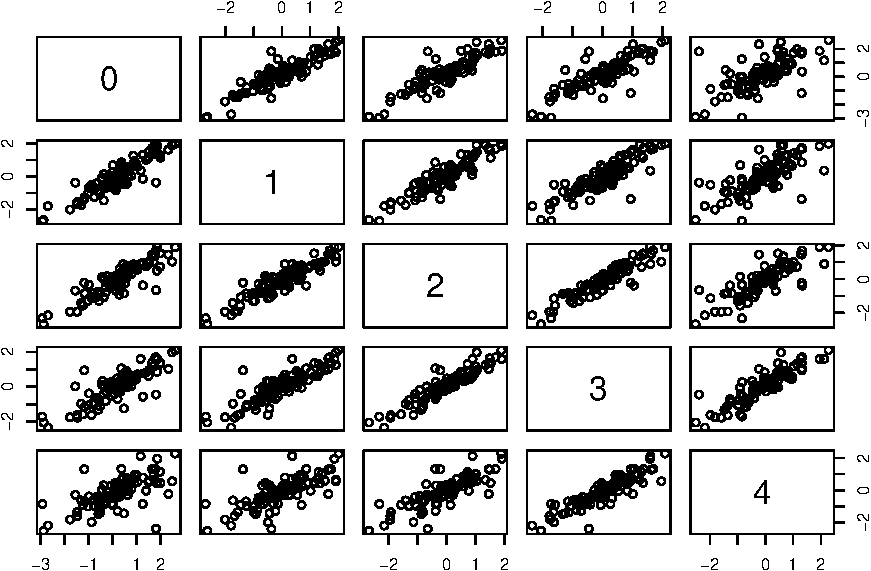
\includegraphics{ProblemSet3_ts_1677791812_files/figure-latex/unnamed-chunk-9-1.pdf}

The model for the variance is a function of the visits.

\begin{Shaded}
\begin{Highlighting}[]
\CommentTok{\# Autocorrelation function}
\NormalTok{autocorr\_fit1 }\OtherTok{\textless{}{-}} \FunctionTok{gls}\NormalTok{(zscores }\SpecialCharTok{\textasciitilde{}}\NormalTok{ age }\SpecialCharTok{+}\NormalTok{ female }\SpecialCharTok{+}\NormalTok{ age}\SpecialCharTok{*}\NormalTok{female, }\AttributeTok{data =}\NormalTok{ d\_clean)}
\CommentTok{\# Run autocorrelation function}
\CommentTok{\# The form argument follows \textasciitilde{} 1 (meaning no covariate) then indicate the ID variable of the individual}
\FunctionTok{ACF}\NormalTok{(autocorr\_fit1, }\AttributeTok{form =} \SpecialCharTok{\textasciitilde{}}   \DecValTok{1} \SpecialCharTok{|}\NormalTok{ id )}
\end{Highlighting}
\end{Shaded}

\begin{verbatim}
##   lag   ACF
## 1   0 1.000
## 2   1 0.879
## 3   2 0.819
## 4   3 0.779
## 5   4 0.657
\end{verbatim}

\hypertarget{constant-variance-assumptions-for-the-residuals}{%
\paragraph{constant variance assumptions for the
residuals}\label{constant-variance-assumptions-for-the-residuals}}

\begin{Shaded}
\begin{Highlighting}[]
\NormalTok{d\_clean }\OtherTok{=} \FunctionTok{mutate}\NormalTok{(d\_clean, }\AttributeTok{r2 =}\NormalTok{ residuals}\SpecialCharTok{\^{}}\DecValTok{2}\NormalTok{)}
\CommentTok{\# Scatterplot of log squared residuals by age,}
\CommentTok{\# ggplot(d\_clean,aes(x=age, y=r2, group = female, color = female)) +}
\CommentTok{\#     geom\_jitter(alpha = 0.5) +}
\CommentTok{\#     theme\_bw() +}
\CommentTok{\#     geom\_smooth() +}
\CommentTok{\#     labs(y="Squared residuasl",x="Age (in months)", color = "Sex")}
\FunctionTok{ggplot}\NormalTok{(d\_clean,}\FunctionTok{aes}\NormalTok{(}\AttributeTok{x=}\NormalTok{age, }\AttributeTok{y=}\NormalTok{r2 )) }\SpecialCharTok{+}
    \FunctionTok{geom\_jitter}\NormalTok{(}\AttributeTok{alpha =} \FloatTok{0.5}\NormalTok{) }\SpecialCharTok{+}
    \FunctionTok{theme\_bw}\NormalTok{() }\SpecialCharTok{+}
    \FunctionTok{geom\_smooth}\NormalTok{() }\SpecialCharTok{+}
    \FunctionTok{labs}\NormalTok{(}\AttributeTok{y=}\StringTok{"Squared residuasl"}\NormalTok{,}\AttributeTok{x=}\StringTok{"Age (in months)"}\NormalTok{ )}
\end{Highlighting}
\end{Shaded}

\begin{verbatim}
## `geom_smooth()` using method = 'loess' and formula = 'y ~ x'
\end{verbatim}

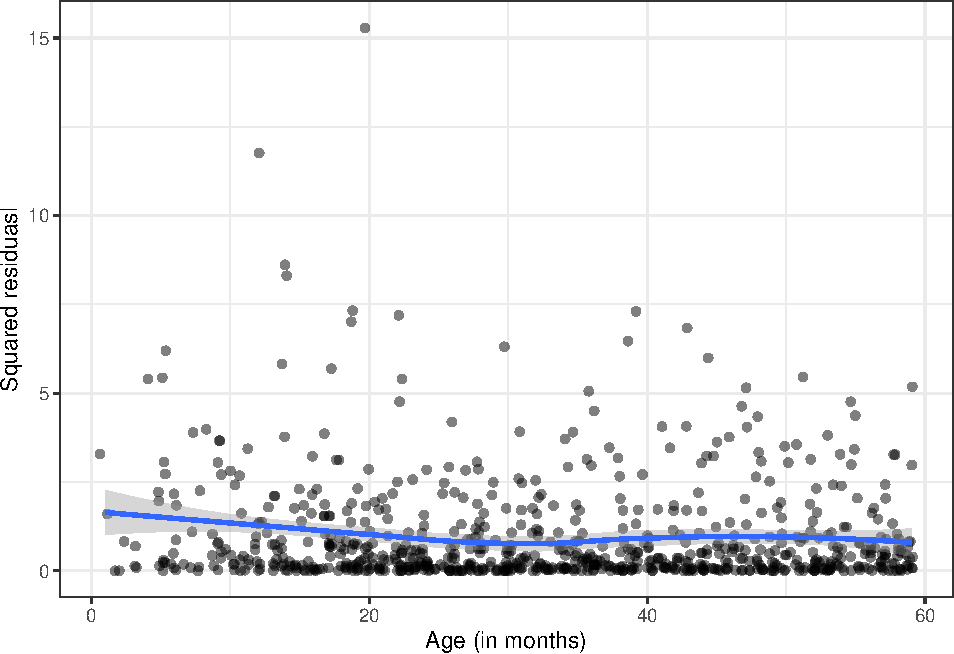
\includegraphics{ProblemSet3_ts_1677791812_files/figure-latex/unnamed-chunk-11-1.pdf}

The variation in the residuals for the female children look roughly the
same over the age. There appears to be a reduction in the variance of
the residuals as age increased to 25 months for male children. So we can
propose to modify our multiple linear regression model to relax the
homoskedasticity assumption and propose a variance model that is a
function of age.

For example our model may be:\\
Var(\(\epsilon_{ij}\))=\(\gamma_0\)+\(\gamma_1\)\textbar(age-25)\textbar(sex
= male)

\hypertarget{based-on-your-model-checking-propose-an-alternative-model-for-the-data-that-can-address-the-first-goal-of-the-analysis-i.e.-determine-if-the-growth-rates-of-children-differ-by-sex-while-satisfying-the-observed-patterns-in-data-with-respect-to-the-mean-model-and-distribution-of-residuals.-note-if-you-modify-the-mean-model-you-may-want-to-iterate-between-model-checking-for-the-mean.}{%
\subsubsection{2.Based on your model checking, propose an alternative
model for the data that can address the first goal of the analysis,
i.e.~determine if the growth rates of children differ by sex while
satisfying the observed patterns in data with respect to the mean model
and distribution of residuals. NOTE: If you modify the mean model, you
may want to iterate between model checking for the
mean.}\label{based-on-your-model-checking-propose-an-alternative-model-for-the-data-that-can-address-the-first-goal-of-the-analysis-i.e.-determine-if-the-growth-rates-of-children-differ-by-sex-while-satisfying-the-observed-patterns-in-data-with-respect-to-the-mean-model-and-distribution-of-residuals.-note-if-you-modify-the-mean-model-you-may-want-to-iterate-between-model-checking-for-the-mean.}}

\begin{Shaded}
\begin{Highlighting}[]
\NormalTok{d\_clean }\OtherTok{\textless{}{-}}\NormalTok{ d\_clean }\SpecialCharTok{|\textgreater{}}
  \FunctionTok{mutate}\NormalTok{(}\AttributeTok{age\_12 =} \FunctionTok{ifelse}\NormalTok{(age}\DecValTok{{-}12}\SpecialCharTok{\textgreater{}}\DecValTok{0}\NormalTok{, age }\SpecialCharTok{{-}}\DecValTok{12}\NormalTok{, }\DecValTok{0}\NormalTok{))}

\NormalTok{model2 }\OtherTok{\textless{}{-}} \FunctionTok{lm}\NormalTok{(zscores}\SpecialCharTok{\textasciitilde{}}\NormalTok{ age }\SpecialCharTok{+}\NormalTok{ age\_12 }\SpecialCharTok{+}\NormalTok{ female }\SpecialCharTok{+}\NormalTok{ age}\SpecialCharTok{*}\NormalTok{female }\SpecialCharTok{+}\NormalTok{ age\_12}\SpecialCharTok{*}\NormalTok{female, }\AttributeTok{data =}\NormalTok{ d\_clean)}
\end{Highlighting}
\end{Shaded}

\hypertarget{assumption-ey-x-x-beta-1}{%
\paragraph{\texorpdfstring{assumption E(Y \textbar X) = X
\(\beta\)}{assumption E(Y \textbar X) = X \textbackslash beta}}\label{assumption-ey-x-x-beta-1}}

checking the mean:

\begin{Shaded}
\begin{Highlighting}[]
\NormalTok{d\_clean}\SpecialCharTok{$}\NormalTok{residuals2 }\OtherTok{=} \FunctionTok{residuals}\NormalTok{(model2)}
\FunctionTok{ggplot}\NormalTok{(d\_clean,}\FunctionTok{aes}\NormalTok{(}\AttributeTok{x=}\NormalTok{age, }\AttributeTok{y=}\NormalTok{residuals2)) }\SpecialCharTok{+}
    \FunctionTok{geom\_jitter}\NormalTok{(}\AttributeTok{alpha =} \FloatTok{0.7}\NormalTok{) }\SpecialCharTok{+}
    \FunctionTok{theme\_bw}\NormalTok{() }\SpecialCharTok{+}
    \FunctionTok{geom\_smooth}\NormalTok{() }\SpecialCharTok{+}
    \FunctionTok{geom\_hline}\NormalTok{(}\AttributeTok{yintercept=}\DecValTok{0}\NormalTok{,}\AttributeTok{color=}\StringTok{"red"}\NormalTok{) }\SpecialCharTok{+}
    \FunctionTok{labs}\NormalTok{(}\AttributeTok{y=}\StringTok{"Residuals: linear spline age"}\NormalTok{,}\AttributeTok{x=}\StringTok{"Age in months"}\NormalTok{) }\SpecialCharTok{+}
    \FunctionTok{scale\_y\_continuous}\NormalTok{(}\AttributeTok{breaks=}\FunctionTok{seq}\NormalTok{(}\SpecialCharTok{{-}}\FloatTok{3.5}\NormalTok{,}\FloatTok{3.5}\NormalTok{,}\FloatTok{0.5}\NormalTok{),}\AttributeTok{limits=}\FunctionTok{c}\NormalTok{(}\SpecialCharTok{{-}}\FloatTok{3.5}\NormalTok{,}\FloatTok{3.5}\NormalTok{)) }\SpecialCharTok{+}
  \FunctionTok{scale\_x\_continuous}\NormalTok{(}\AttributeTok{breaks=}\FunctionTok{seq}\NormalTok{(}\DecValTok{0}\NormalTok{,}\DecValTok{60}\NormalTok{,}\DecValTok{6}\NormalTok{),}\AttributeTok{limits=}\FunctionTok{c}\NormalTok{(}\DecValTok{0}\NormalTok{,}\DecValTok{60}\NormalTok{))}
\end{Highlighting}
\end{Shaded}

\begin{verbatim}
## `geom_smooth()` using method = 'loess' and formula = 'y ~ x'
\end{verbatim}

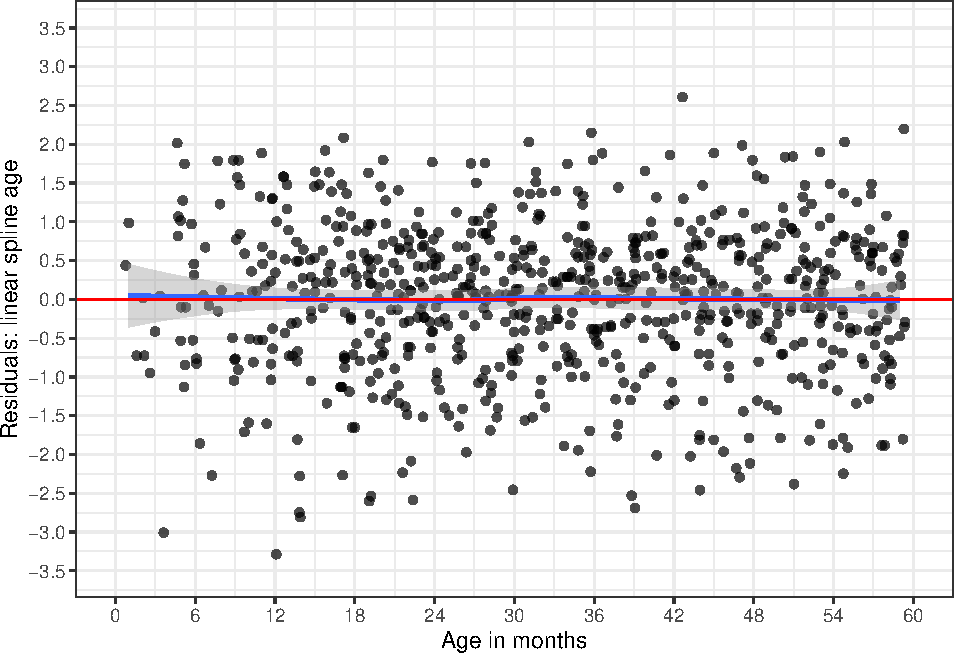
\includegraphics{ProblemSet3_ts_1677791812_files/figure-latex/unnamed-chunk-13-1.pdf}

\hypertarget{independence-assumption-1}{%
\paragraph{Independence assumption}\label{independence-assumption-1}}

Visualizing autocorrelation using a scatterplot matrix

\begin{Shaded}
\begin{Highlighting}[]
\CommentTok{\# Retrieve only the zscores, age, and Model 1}
\NormalTok{d\_wide2 }\OtherTok{\textless{}{-}}\NormalTok{ d\_clean }\SpecialCharTok{|\textgreater{}}
  \FunctionTok{select}\NormalTok{(residuals2, fuvisit, id) }\SpecialCharTok{|\textgreater{}}
  \FunctionTok{pivot\_wider}\NormalTok{(}\AttributeTok{id\_cols =} \StringTok{"id"}\NormalTok{,}
              \AttributeTok{names\_from =} \StringTok{"fuvisit"}\NormalTok{,}
              \AttributeTok{values\_from =} \StringTok{"residuals2"}\NormalTok{)}

\CommentTok{\# View the wide data}
\FunctionTok{head}\NormalTok{(d\_wide2, }\AttributeTok{n =} \DecValTok{3}\NormalTok{)}
\end{Highlighting}
\end{Shaded}

\begin{verbatim}
## # A tibble: 3 x 6
##       id   `0`    `1`     `2`     `3`    `4`
##    <int> <dbl>  <dbl>   <dbl>   <dbl>  <dbl>
## 1 120011 0.587  0.193  0.0186  0.0842 NA    
## 2 120012 0.678 NA     NA      NA      NA    
## 3 120021 1.23   1.30   1.02    0.707   0.604
\end{verbatim}

\begin{Shaded}
\begin{Highlighting}[]
\CommentTok{\# Use wide format of the data}
\FunctionTok{cor}\NormalTok{(d\_wide2[,}\FunctionTok{c}\NormalTok{(}\DecValTok{2}\SpecialCharTok{:}\DecValTok{6}\NormalTok{)])}
\end{Highlighting}
\end{Shaded}

\begin{verbatim}
##    0  1  2  3  4
## 0  1 NA NA NA NA
## 1 NA  1 NA NA NA
## 2 NA NA  1 NA NA
## 3 NA NA NA  1 NA
## 4 NA NA NA NA  1
\end{verbatim}

\begin{Shaded}
\begin{Highlighting}[]
\FunctionTok{pairs}\NormalTok{(d\_wide2[,}\FunctionTok{c}\NormalTok{(}\DecValTok{2}\SpecialCharTok{:}\DecValTok{6}\NormalTok{)])}
\end{Highlighting}
\end{Shaded}

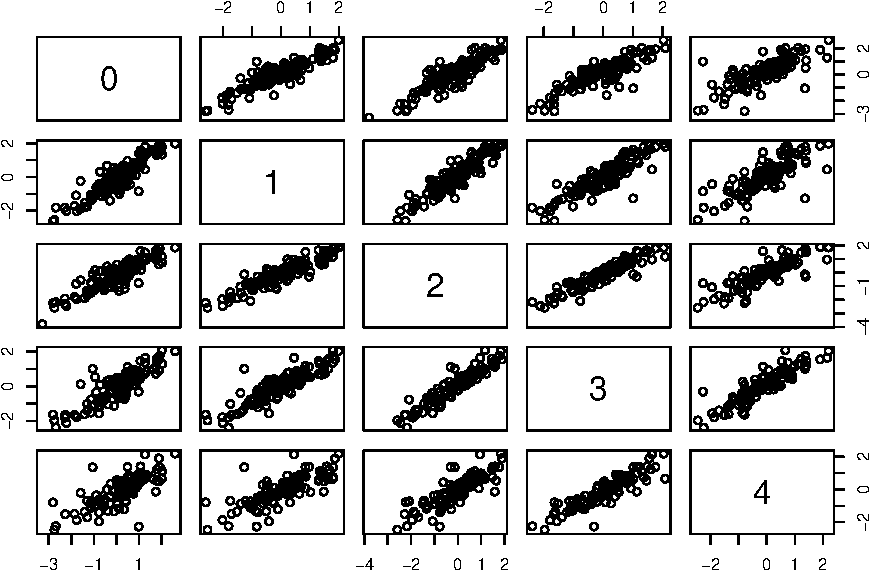
\includegraphics{ProblemSet3_ts_1677791812_files/figure-latex/unnamed-chunk-14-1.pdf}

The model for the variance is a function of the visits.

\begin{Shaded}
\begin{Highlighting}[]
\CommentTok{\# Autocorrelation function}
\NormalTok{autocorr\_fit2 }\OtherTok{\textless{}{-}} \FunctionTok{gls}\NormalTok{(zscores }\SpecialCharTok{\textasciitilde{}}\NormalTok{ age }\SpecialCharTok{+}\NormalTok{ age\_12 }\SpecialCharTok{+}\NormalTok{ female }\SpecialCharTok{+}\NormalTok{ age}\SpecialCharTok{*}\NormalTok{female }\SpecialCharTok{+}\NormalTok{ age\_12}\SpecialCharTok{*}\NormalTok{female, }\AttributeTok{data =}\NormalTok{ d\_clean)}
\CommentTok{\# Run autocorrelation function}
\CommentTok{\# The form argument follows \textasciitilde{} 1 (meaning no covariate) then indicate the ID variable of the individual}
\FunctionTok{ACF}\NormalTok{(autocorr\_fit2, }\AttributeTok{form =} \SpecialCharTok{\textasciitilde{}}   \DecValTok{1} \SpecialCharTok{|}\NormalTok{ id )}
\end{Highlighting}
\end{Shaded}

\begin{verbatim}
##   lag   ACF
## 1   0 1.000
## 2   1 0.883
## 3   2 0.829
## 4   3 0.803
## 5   4 0.713
\end{verbatim}

\hypertarget{constant-variance-assumptions-for-the-residuals-1}{%
\paragraph{constant variance assumptions for the
residuals}\label{constant-variance-assumptions-for-the-residuals-1}}

\begin{Shaded}
\begin{Highlighting}[]
\NormalTok{d\_clean }\OtherTok{=} \FunctionTok{mutate}\NormalTok{(d\_clean, }\AttributeTok{r2\_new =}\NormalTok{ residuals2}\SpecialCharTok{\^{}}\DecValTok{2}\NormalTok{)}
\CommentTok{\# Scatterplot of log squared residuals by age,}
\FunctionTok{ggplot}\NormalTok{(d\_clean,}\FunctionTok{aes}\NormalTok{(}\AttributeTok{x=}\NormalTok{age, }\AttributeTok{y=}\NormalTok{r2\_new, }\AttributeTok{group =}\NormalTok{ female, }\AttributeTok{color =}\NormalTok{ female)) }\SpecialCharTok{+}
    \FunctionTok{geom\_jitter}\NormalTok{(}\AttributeTok{alpha =} \FloatTok{0.5}\NormalTok{) }\SpecialCharTok{+}
    \FunctionTok{theme\_bw}\NormalTok{() }\SpecialCharTok{+}
    \FunctionTok{geom\_smooth}\NormalTok{() }\SpecialCharTok{+}
    \FunctionTok{labs}\NormalTok{(}\AttributeTok{y=}\StringTok{"Squared residuasl"}\NormalTok{,}\AttributeTok{x=}\StringTok{"Age (in months)"}\NormalTok{, }\AttributeTok{color =} \StringTok{"Sex"}\NormalTok{)}
\end{Highlighting}
\end{Shaded}

\begin{verbatim}
## `geom_smooth()` using method = 'loess' and formula = 'y ~ x'
\end{verbatim}

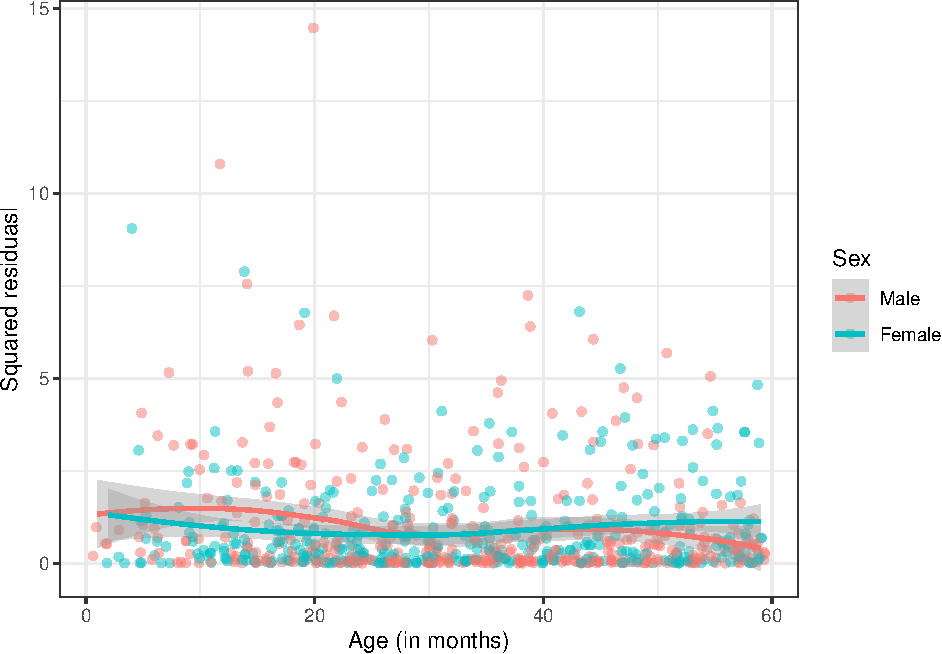
\includegraphics{ProblemSet3_ts_1677791812_files/figure-latex/unnamed-chunk-16-1.pdf}

\hypertarget{resicual-are-normally-distributed}{%
\paragraph{resicual are normally
distributed}\label{resicual-are-normally-distributed}}

\begin{Shaded}
\begin{Highlighting}[]
\FunctionTok{plot}\NormalTok{(model2)}
\end{Highlighting}
\end{Shaded}

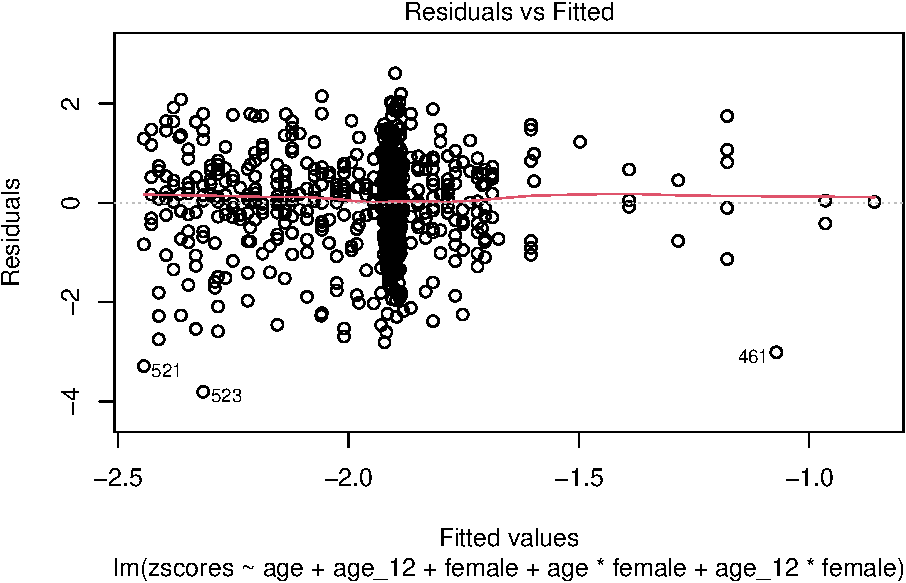
\includegraphics{ProblemSet3_ts_1677791812_files/figure-latex/unnamed-chunk-17-1.pdf}
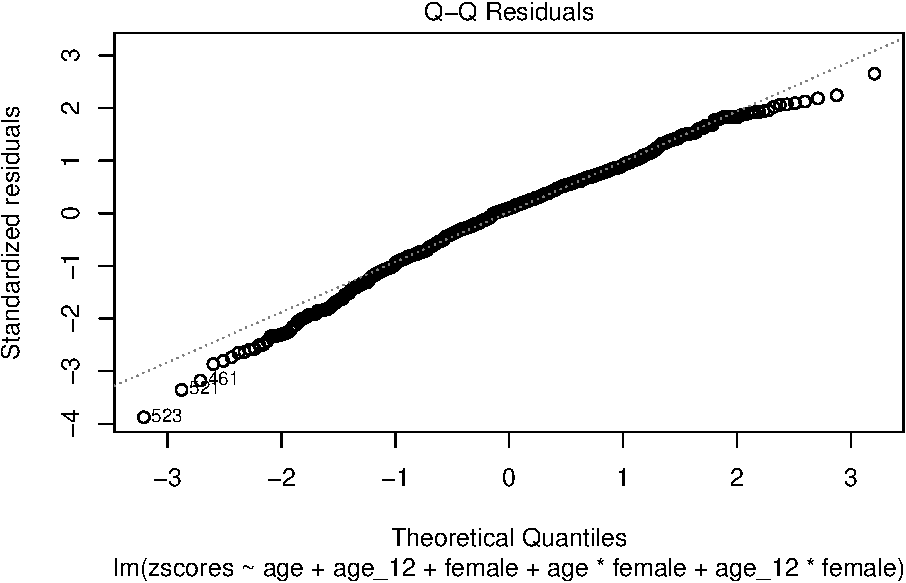
\includegraphics{ProblemSet3_ts_1677791812_files/figure-latex/unnamed-chunk-17-2.pdf}
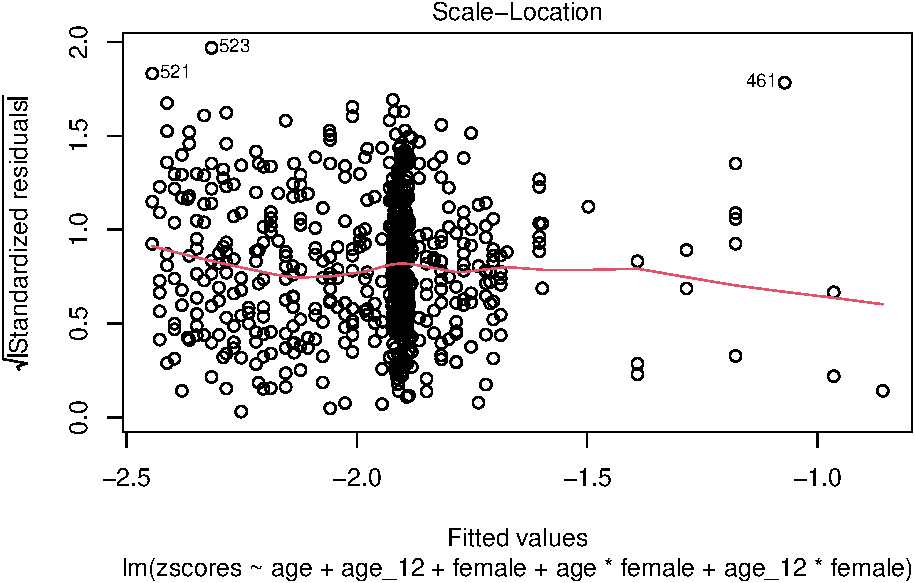
\includegraphics{ProblemSet3_ts_1677791812_files/figure-latex/unnamed-chunk-17-3.pdf}
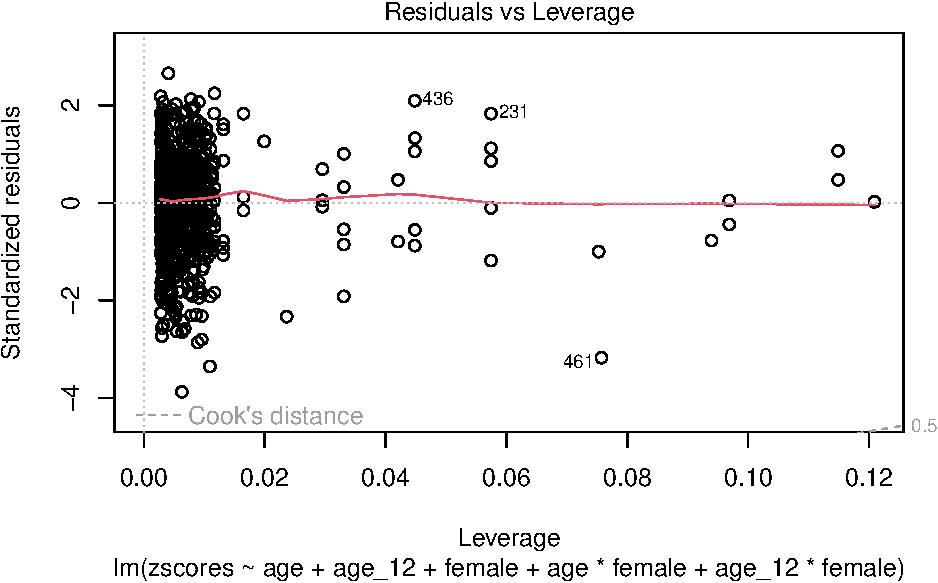
\includegraphics{ProblemSet3_ts_1677791812_files/figure-latex/unnamed-chunk-17-4.pdf}

\hypertarget{part-iii-marginal-model-for-longitudinal-data}{%
\section{Part III: Marginal model for longitudinal
data}\label{part-iii-marginal-model-for-longitudinal-data}}

\hypertarget{use-the-gls-function-in-r-to-fit-the-model-you-proposed-in-part-i.}{%
\subsubsection{1.Use the gls function in R to fit the model you proposed
in Part
I.}\label{use-the-gls-function-in-r-to-fit-the-model-you-proposed-in-part-i.}}

\begin{Shaded}
\begin{Highlighting}[]
\CommentTok{\# AR(1): }
\NormalTok{model\_AR }\OtherTok{\textless{}{-}} \FunctionTok{gls}\NormalTok{(zscores }\SpecialCharTok{\textasciitilde{}}\NormalTok{age }\SpecialCharTok{+}\NormalTok{ age\_12 }\SpecialCharTok{+}\NormalTok{ female }\SpecialCharTok{+}\NormalTok{ age}\SpecialCharTok{*}\NormalTok{female }\SpecialCharTok{+}\NormalTok{ age\_12}\SpecialCharTok{*}\NormalTok{female, }\AttributeTok{data =}\NormalTok{ d\_clean, }\AttributeTok{correlation =} \FunctionTok{corAR1}\NormalTok{(}\AttributeTok{form=} \SpecialCharTok{\textasciitilde{}}\NormalTok{fuvisit}\SpecialCharTok{|}\NormalTok{id), }\AttributeTok{weights =} \FunctionTok{varFunc}\NormalTok{(}\SpecialCharTok{\textasciitilde{}}\FunctionTok{as.numeric}\NormalTok{(female)))}
\FunctionTok{summary}\NormalTok{(model\_AR)}\SpecialCharTok{$}\NormalTok{tTable}
\end{Highlighting}
\end{Shaded}

\begin{verbatim}
##                        Value Std.Error t-value  p-value
## (Intercept)         -1.17588    0.2282  -5.154 3.28e-07
## age                 -0.09256    0.0180  -5.134 3.64e-07
## age_12               0.10202    0.0191   5.340 1.24e-07
## femaleFemale         0.35031    0.4144   0.845 3.98e-01
## age:femaleFemale     0.00896    0.0333   0.269 7.88e-01
## age_12:femaleFemale -0.02286    0.0351  -0.651 5.15e-01
\end{verbatim}

\begin{Shaded}
\begin{Highlighting}[]
\CommentTok{\# \# Toeplitz: }
\CommentTok{\# model\_Toep \textless{}{-} gls(zscores \textasciitilde{}age + age\_12 + female + age*female + age\_12*female, data = d\_clean, correlation = corARMA(form= \textasciitilde{}fuvisit|id, p=4, q=0))}
\CommentTok{\# summary(model\_Toep)$tTable}
\end{Highlighting}
\end{Shaded}

\hypertarget{from-the-fit-of-the-model-compute-the-estimated-correpsilon_i1-epsilon_ij-for-j-2-3-4-5-where-the-follow-up-visits-fuvisit-have-values-0-baseline-j1-and-1-2-3-4-representing-the-4-follow-up-visits-each-4-months-apartj-2-3-4-5.-compare-these-model-based-correlation-estimates-to-those-you-computed-in-part-ii-question1.}{%
\subsubsection{\texorpdfstring{2.From the fit of the model, compute the
estimated Corr(\(\epsilon_{i1}\), \(\epsilon_{ij}\)) for j = 2, 3, 4, 5
where the follow-up visits (fuvisit) have values 0 (baseline, j=1) and
1, 2, 3, 4 (representing the 4 follow-up visits each 4 months apart,j =
2, 3, 4, 5). Compare these model-based correlation estimates to those
you computed in Part II
Question1.}{2.From the fit of the model, compute the estimated Corr(\textbackslash epsilon\_\{i1\}, \textbackslash epsilon\_\{ij\}) for j = 2, 3, 4, 5 where the follow-up visits (fuvisit) have values 0 (baseline, j=1) and 1, 2, 3, 4 (representing the 4 follow-up visits each 4 months apart,j = 2, 3, 4, 5). Compare these model-based correlation estimates to those you computed in Part II Question1.}}\label{from-the-fit-of-the-model-compute-the-estimated-correpsilon_i1-epsilon_ij-for-j-2-3-4-5-where-the-follow-up-visits-fuvisit-have-values-0-baseline-j1-and-1-2-3-4-representing-the-4-follow-up-visits-each-4-months-apartj-2-3-4-5.-compare-these-model-based-correlation-estimates-to-those-you-computed-in-part-ii-question1.}}

\begin{Shaded}
\begin{Highlighting}[]
\CommentTok{\# AR(1): }
\NormalTok{female.V }\OtherTok{=} \FunctionTok{getVarCov}\NormalTok{(model\_AR, }\AttributeTok{individual=}\DecValTok{3}\NormalTok{)}
\FunctionTok{cov2cor}\NormalTok{(female.V)}
\end{Highlighting}
\end{Shaded}

\begin{verbatim}
## Marginal variance covariance matrix
##       [,1]  [,2]  [,3]  [,4]  [,5]
## [1,] 1.000 0.912 0.831 0.758 0.691
## [2,] 0.912 1.000 0.912 0.831 0.758
## [3,] 0.831 0.912 1.000 0.912 0.831
## [4,] 0.758 0.831 0.912 1.000 0.912
## [5,] 0.691 0.758 0.831 0.912 1.000
##   Standard Deviations: 1 1 1 1 1
\end{verbatim}

\begin{Shaded}
\begin{Highlighting}[]
\NormalTok{male.V }\OtherTok{=} \FunctionTok{getVarCov}\NormalTok{(model\_AR,}\AttributeTok{individual=}\DecValTok{7}\NormalTok{)}
\FunctionTok{cov2cor}\NormalTok{(male.V)}
\end{Highlighting}
\end{Shaded}

\begin{verbatim}
## Marginal variance covariance matrix
##       [,1]  [,2]  [,3]  [,4]  [,5]
## [1,] 1.000 0.912 0.831 0.758 0.691
## [2,] 0.912 1.000 0.912 0.831 0.758
## [3,] 0.831 0.912 1.000 0.912 0.831
## [4,] 0.758 0.831 0.912 1.000 0.912
## [5,] 0.691 0.758 0.831 0.912 1.000
##   Standard Deviations: 1 1 1 1 1
\end{verbatim}

\begin{Shaded}
\begin{Highlighting}[]
\CommentTok{\# Toeplitz: }
\CommentTok{\# getVarCov(model\_Toep, individual=1)}
\CommentTok{\# round(cov2cor(getVarCov(model\_Toep, individual=1)),3)}
\end{Highlighting}
\end{Shaded}

For time point 1 (baseline, j=1) to time point 2 (j=2), the AR(1) model
estimates correlation of 0.912, while the previously computed
correlation was 0.904. For time point 1 (baseline, j=1) to time point 3
(j=3), the AR(1) model estimates the correlation as 0.831, in comparison
to the previously one 0.883. Correlation between time point 1 and 4 was
0.758 in AR(1) model, and 0.836 in previous model. This AR(1) model
provides a more smooth decrease in correlation over time, which is
characteristic of the exponential decay pattern typical of AR(1)
processes.

\hypertarget{conduct-a-wald-test-to-address-the-overall-goal-of-the-analysis-i.e.-to-determine-if-the-average-growth-rates-of-children-differ-by-sex.}{%
\subsubsection{3. Conduct a Wald test to address the overall goal of the
analysis; i.e.~to determine if the average growth rates of children
differ by
sex.}\label{conduct-a-wald-test-to-address-the-overall-goal-of-the-analysis-i.e.-to-determine-if-the-average-growth-rates-of-children-differ-by-sex.}}

\begin{Shaded}
\begin{Highlighting}[]
\FunctionTok{library}\NormalTok{(nlme)}

\CommentTok{\# Extract estimated regression coefficients}
\NormalTok{beta\_hat }\OtherTok{\textless{}{-}} \FunctionTok{coef}\NormalTok{(model\_AR)}

\CommentTok{\# estimated variance of $\textbackslash{}beta\_hat$ }
\NormalTok{V\_beta\_hat }\OtherTok{\textless{}{-}} \FunctionTok{summary}\NormalTok{(model\_AR)}\SpecialCharTok{$}\NormalTok{varBeta}

\NormalTok{C }\OtherTok{\textless{}{-}} \FunctionTok{matrix}\NormalTok{(}\FunctionTok{c}\NormalTok{(}\DecValTok{0}\NormalTok{, }\DecValTok{0}\NormalTok{, }\DecValTok{0}\NormalTok{, }\DecValTok{1}\NormalTok{, }\DecValTok{0}\NormalTok{, }\DecValTok{0}\NormalTok{,   }\CommentTok{\# for female}
              \DecValTok{0}\NormalTok{, }\DecValTok{0}\NormalTok{, }\DecValTok{0}\NormalTok{, }\DecValTok{0}\NormalTok{, }\DecValTok{1}\NormalTok{, }\DecValTok{0}\NormalTok{,   }\CommentTok{\# for age:female}
              \DecValTok{0}\NormalTok{, }\DecValTok{0}\NormalTok{, }\DecValTok{0}\NormalTok{, }\DecValTok{0}\NormalTok{, }\DecValTok{0}\NormalTok{, }\DecValTok{1}\NormalTok{),  }\CommentTok{\# for age\_12:female}
            \AttributeTok{nrow =} \DecValTok{3}\NormalTok{, }\AttributeTok{byrow =} \ConstantTok{TRUE}\NormalTok{)}


\CommentTok{\# Calculate the Wald test statistic Q}
\NormalTok{Q }\OtherTok{\textless{}{-}} \FunctionTok{t}\NormalTok{(C }\SpecialCharTok{\%*\%}\NormalTok{ beta\_hat) }\SpecialCharTok{\%*\%} \FunctionTok{solve}\NormalTok{(C }\SpecialCharTok{\%*\%}\NormalTok{ V\_beta\_hat }\SpecialCharTok{\%*\%} \FunctionTok{t}\NormalTok{(C)) }\SpecialCharTok{\%*\%}\NormalTok{ (C }\SpecialCharTok{\%*\%}\NormalTok{ beta\_hat)}

\CommentTok{\# Degrees of freedom for the chi{-}squared distribution}
\NormalTok{df }\OtherTok{\textless{}{-}} \FunctionTok{nrow}\NormalTok{(C)}

\CommentTok{\# Calculate p{-}value from the chi{-}squared distribution}
\NormalTok{p\_value }\OtherTok{\textless{}{-}} \DecValTok{1} \SpecialCharTok{{-}} \FunctionTok{pchisq}\NormalTok{(Q, df)}

\CommentTok{\# Output the test statistic and p{-}value}
\FunctionTok{list}\NormalTok{(}\AttributeTok{Wald\_test\_statistic =}\NormalTok{ Q, }\AttributeTok{p\_value =}\NormalTok{ p\_value)}
\end{Highlighting}
\end{Shaded}

\begin{verbatim}
## $Wald_test_statistic
##      [,1]
## [1,] 4.74
## 
## $p_value
##       [,1]
## [1,] 0.192
\end{verbatim}

The Wald test statistic is 4.74 and p-value is 0.192. We fail to reject
the null hypothesis that the average growth rates are the same by sex.

\hypertarget{part-iv-sensitivity-analysis-for-the-marginal-model-results}{%
\section{Part IV: Sensitivity analysis for the marginal model
results}\label{part-iv-sensitivity-analysis-for-the-marginal-model-results}}

\hypertarget{section}{%
\subsection{1.}\label{section}}

\hypertarget{a.-show-that-the-robust-variance-estimator-is-equal-to-the-generalized-least-squares-variance-estimator-when-epsilo-is-correctly-specified}{%
\paragraph{a. Show that the robust variance estimator is equal to the
generalized least squares variance estimator when epsilo is correctly
specified}\label{a.-show-that-the-robust-variance-estimator-is-equal-to-the-generalized-least-squares-variance-estimator-when-epsilo-is-correctly-specified}}

\begin{figure}
\centering
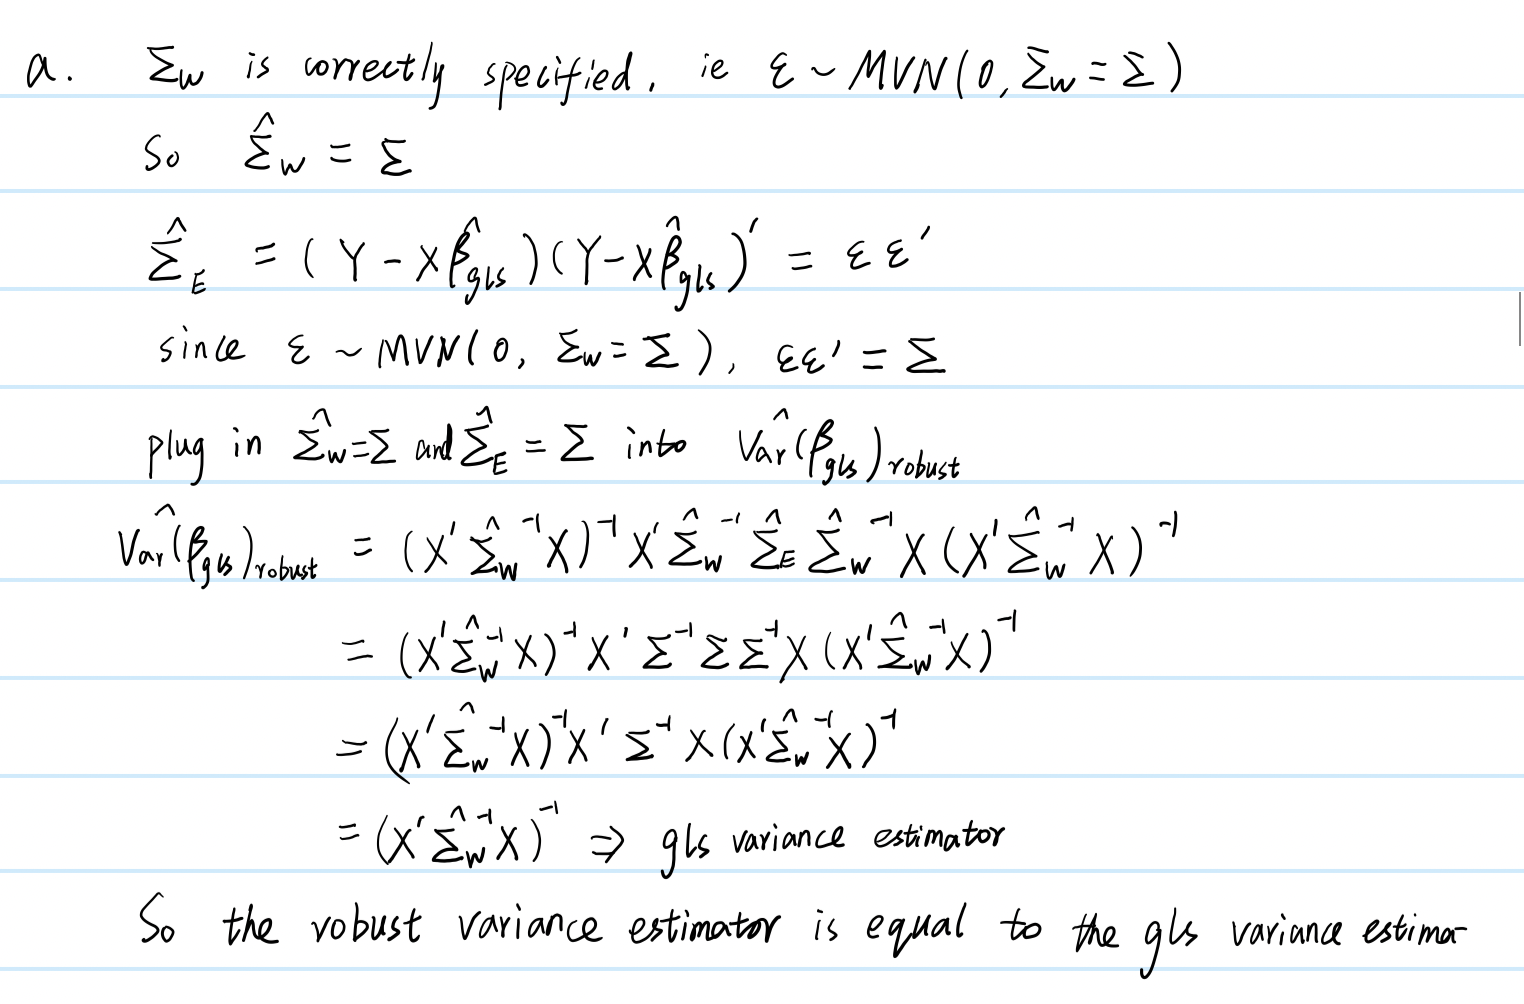
\includegraphics[width=5.20833in,height=\textheight]{images/problemset3.png}
\caption{Part 4-1}
\end{figure}

\hypertarget{b.-for-the-model-you-fit-in-part-iii-question1-obtain-the-robust-standard-error-estimates-using-the-huber-white-sandwich-estimator.-compare-the-estimated-model-based-and-robust-standard-errors.}{%
\paragraph{b. For the model you fit in Part III Question1, obtain the
robust standard error estimates using the Huber-White sandwich
estimator. Compare the estimated model based and robust standard
errors.}\label{b.-for-the-model-you-fit-in-part-iii-question1-obtain-the-robust-standard-error-estimates-using-the-huber-white-sandwich-estimator.-compare-the-estimated-model-based-and-robust-standard-errors.}}

\begin{Shaded}
\begin{Highlighting}[]
\CommentTok{\# install.packages("clubSandwich")}
\FunctionTok{library}\NormalTok{(clubSandwich)}
\end{Highlighting}
\end{Shaded}

\begin{verbatim}
## Registered S3 method overwritten by 'clubSandwich':
##   method    from    
##   bread.mlm sandwich
\end{verbatim}

\begin{Shaded}
\begin{Highlighting}[]
\CommentTok{\# Fit the model}
\NormalTok{model\_AR }\OtherTok{\textless{}{-}} \FunctionTok{gls}\NormalTok{(zscores }\SpecialCharTok{\textasciitilde{}}\NormalTok{age }\SpecialCharTok{+}\NormalTok{ age\_12 }\SpecialCharTok{+}\NormalTok{ female }\SpecialCharTok{+}\NormalTok{ age}\SpecialCharTok{*}\NormalTok{female }\SpecialCharTok{+}\NormalTok{ age\_12}\SpecialCharTok{*}\NormalTok{female, }\AttributeTok{data =}\NormalTok{ d\_clean, }\AttributeTok{correlation =} \FunctionTok{corAR1}\NormalTok{(}\AttributeTok{form=} \SpecialCharTok{\textasciitilde{}}\NormalTok{fuvisit}\SpecialCharTok{|}\NormalTok{id), }\AttributeTok{weights =} \FunctionTok{varFunc}\NormalTok{(}\SpecialCharTok{\textasciitilde{}}\FunctionTok{as.numeric}\NormalTok{(female)))}

\CommentTok{\# Estimate robust standard errors using the cluster{-}robust sandwich estimator}
\CommentTok{\# This is the robust estimate of Var{-}hat(beta{-}hat)}
\NormalTok{vcov.rob }\OtherTok{\textless{}{-}} \FunctionTok{vcovCR}\NormalTok{(model\_AR, }\AttributeTok{cluster =}\NormalTok{ d\_clean}\SpecialCharTok{$}\NormalTok{id, }\AttributeTok{type =} \StringTok{"CR0"}\NormalTok{)}
\CommentTok{\# Save the results for testing each individual coefficient}
\NormalTok{clubsand }\OtherTok{\textless{}{-}} \FunctionTok{coef\_test}\NormalTok{(model\_AR, }\AttributeTok{vcov =}\NormalTok{ vcov.rob)}
\CommentTok{\# Compare the standard errors}
\FunctionTok{summary}\NormalTok{(model\_AR)}\SpecialCharTok{$}\NormalTok{tTable}
\end{Highlighting}
\end{Shaded}

\begin{verbatim}
##                        Value Std.Error t-value  p-value
## (Intercept)         -1.17588    0.2282  -5.154 3.28e-07
## age                 -0.09256    0.0180  -5.134 3.64e-07
## age_12               0.10202    0.0191   5.340 1.24e-07
## femaleFemale         0.35031    0.4144   0.845 3.98e-01
## age:femaleFemale     0.00896    0.0333   0.269 7.88e-01
## age_12:femaleFemale -0.02286    0.0351  -0.651 5.15e-01
\end{verbatim}

\begin{Shaded}
\begin{Highlighting}[]
\NormalTok{clubsand}
\end{Highlighting}
\end{Shaded}

\begin{verbatim}
##                Coef. Estimate     SE t-stat d.f. (Satt) p-val (Satt) Sig.
##          (Intercept) -1.17588 0.3509 -3.351        16.0      0.00407   **
##                  age -0.09256 0.0276 -3.356        13.0      0.00518   **
##               age_12  0.10202 0.0281  3.636        15.4      0.00235   **
##         femaleFemale  0.35031 0.4340  0.807        26.3      0.42681     
##     age:femaleFemale  0.00896 0.0331  0.271        21.5      0.78895     
##  age_12:femaleFemale -0.02286 0.0337 -0.679        25.1      0.50343
\end{verbatim}

For intercept, The model-based standard error is 0.2282, while the
robust standard error is 0.3509. For ``age'' term, the model-based
standard error is 0.0180, and the robust is 0.0276. For ``age\_12'' and
``female'' terms, the model-based standard error are all smaller than
the robust one. The robust standard errors are larger than the
model-based standard errors, this suggests that the model-based errors
may be underestimating the true variability in the coefficients due to
potential violations of the model assumptions (such as non-constant
variance or correlations not being correctly modeled).

\hypertarget{c.-using-the-results-of-a.-and-b.-above-do-the-data-support-or-not-support-your-working-model-for-the-variancecovariance-of-the-residuals}{%
\paragraph{c.~Using the results of a. and b. above, do the data support
or not support your working model for the variance/covariance of the
residuals?}\label{c.-using-the-results-of-a.-and-b.-above-do-the-data-support-or-not-support-your-working-model-for-the-variancecovariance-of-the-residuals}}

The robust standard errors for most coefficients are larger than the
model-based standard errors. That suggests that the working model
assumptions for the variance/covariance of the residuals may not be
fully appropriate. For the interaction terms, the robust and model-based
standard errors are very similar, suggesting that the working model may
adequately capture the variance/covariance structure for these specific
terms. In conclusion, the data do not fully support the working model
for the variance/covariance of the residuals.

\hypertarget{d.-use-the-robust-variance-estimate-for-you-obtained-called-vcov.rob-in-the-code-above-and-repeat-the-wald-test-you-conducted-in-part-iii-question-3.-are-the-results-of-the-wald-tests-the-same-or-different}{%
\paragraph{d.~Use the robust variance estimate for you obtained (called
vcov.rob in the code above) and repeat the Wald test you conducted in
Part III Question 3. Are the results of the Wald tests the same or
different?}\label{d.-use-the-robust-variance-estimate-for-you-obtained-called-vcov.rob-in-the-code-above-and-repeat-the-wald-test-you-conducted-in-part-iii-question-3.-are-the-results-of-the-wald-tests-the-same-or-different}}

\begin{Shaded}
\begin{Highlighting}[]
\CommentTok{\# Calculate the Wald test statistic using the robust variance{-}covariance matrix}
\NormalTok{Q\_robust }\OtherTok{\textless{}{-}} \FunctionTok{t}\NormalTok{(C }\SpecialCharTok{\%*\%} \FunctionTok{coef}\NormalTok{(model\_AR)) }\SpecialCharTok{\%*\%} \FunctionTok{solve}\NormalTok{(C }\SpecialCharTok{\%*\%}\NormalTok{ vcov.rob }\SpecialCharTok{\%*\%} \FunctionTok{t}\NormalTok{(C)) }\SpecialCharTok{\%*\%}\NormalTok{ (C }\SpecialCharTok{\%*\%} \FunctionTok{coef}\NormalTok{(model\_AR))}

\CommentTok{\# Degrees of freedom: number of restrictions being tested, equal to the number of rows in C}
\NormalTok{df\_robust }\OtherTok{\textless{}{-}} \FunctionTok{nrow}\NormalTok{(C)}

\CommentTok{\# Calculate the p{-}value from the chi{-}squared distribution}
\NormalTok{p\_value\_robust }\OtherTok{\textless{}{-}} \DecValTok{1} \SpecialCharTok{{-}} \FunctionTok{pchisq}\NormalTok{(Q\_robust, df\_robust)}

\CommentTok{\# Output the Wald test statistic and p{-}value}
\FunctionTok{list}\NormalTok{(}\AttributeTok{Wald\_test\_statistic\_robust =}\NormalTok{ Q\_robust, }\AttributeTok{p\_value\_robust =}\NormalTok{ p\_value\_robust)}
\end{Highlighting}
\end{Shaded}

\begin{verbatim}
## $Wald_test_statistic_robust
##      [,1]
## [1,] 6.01
## 
## $p_value_robust
##       [,1]
## [1,] 0.111
\end{verbatim}

Use the robust variance estimate, the Wald test statistic is 6.01 and
p-value is 0.111. We fail to reject the null hypothesis that the average
growth rates are the same by sex. The statistic are different from the
Wald test conducted using the variance estimated by the GLS model, but
they both fail to reject the null.

\hypertarget{instead-of-modelling-the-variancecovariance-of-the-within-subject-residuals-you-could-assume-an-independence-working-model-with-constant-variance-i.e.-fit-the-model-using-ordinary-least-squares-and-apply-a-robust-variance-estimate-for-for-inference-on-.}{%
\subsection{2.Instead of modelling the variance/covariance of the within
subject residuals, you could assume an independence working model with
constant variance, i.e.~fit the model using ordinary least squares, and
apply a robust variance estimate for for inference on
.}\label{instead-of-modelling-the-variancecovariance-of-the-within-subject-residuals-you-could-assume-an-independence-working-model-with-constant-variance-i.e.-fit-the-model-using-ordinary-least-squares-and-apply-a-robust-variance-estimate-for-for-inference-on-.}}

\hypertarget{a.use-the-lm-command-to-refit-your-model-under-working-independence-and-constant-variance-then-obtain-a-robust-variance-estimate-for}{%
\paragraph{a.Use the lm command to refit your model under working
independence and constant variance; then obtain a robust variance
estimate
for}\label{a.use-the-lm-command-to-refit-your-model-under-working-independence-and-constant-variance-then-obtain-a-robust-variance-estimate-for}}

\begin{Shaded}
\begin{Highlighting}[]
\CommentTok{\# Fit the ordinary least squares model}
\NormalTok{fit.ols }\OtherTok{\textless{}{-}} \FunctionTok{lm}\NormalTok{(zscores}\SpecialCharTok{\textasciitilde{}}\NormalTok{ age }\SpecialCharTok{+}\NormalTok{ age\_12 }\SpecialCharTok{+}\NormalTok{ female }\SpecialCharTok{+}\NormalTok{ age}\SpecialCharTok{*}\NormalTok{female }\SpecialCharTok{+}\NormalTok{ age\_12}\SpecialCharTok{*}\NormalTok{female, }\AttributeTok{data =}\NormalTok{ d\_clean)}
\CommentTok{\# Get the robust variance estimate}
\NormalTok{vcov.rob.ols }\OtherTok{\textless{}{-}} \FunctionTok{vcovCR}\NormalTok{(fit.ols, }\AttributeTok{cluster =}\NormalTok{ d\_clean}\SpecialCharTok{$}\NormalTok{id, }\AttributeTok{type =} \StringTok{"CR0"}\NormalTok{)}
\CommentTok{\# Save the results for testing each individual coefficient}
\NormalTok{clubsand.ols }\OtherTok{\textless{}{-}} \FunctionTok{coef\_test}\NormalTok{(fit.ols, }\AttributeTok{vcov =}\NormalTok{ vcov.rob.ols)}
\CommentTok{\# Compare the standard errors for the estimated coefficients}
\FunctionTok{summary}\NormalTok{(fit.ols)}\SpecialCharTok{$}\NormalTok{coeff}
\end{Highlighting}
\end{Shaded}

\begin{verbatim}
##                     Estimate Std. Error t value Pr(>|t|)
## (Intercept)          -1.5203     0.3660  -4.154 3.65e-05
## age                  -0.0770     0.0334  -2.304 2.15e-02
## age_12                0.0931     0.0351   2.653 8.16e-03
## femaleFemale          0.8748     0.5533   1.581 1.14e-01
## age:femaleFemale     -0.0295     0.0501  -0.589 5.56e-01
## age_12:femaleFemale   0.0142     0.0524   0.272 7.86e-01
\end{verbatim}

\begin{Shaded}
\begin{Highlighting}[]
\NormalTok{clubsand.ols}
\end{Highlighting}
\end{Shaded}

\begin{verbatim}
##                Coef. Estimate     SE t-stat d.f. (Satt) p-val (Satt) Sig.
##          (Intercept)  -1.5203 0.3639 -4.178        9.57      0.00209   **
##                  age  -0.0770 0.0338 -2.279       12.13      0.04155    *
##               age_12   0.0931 0.0370  2.513       13.86      0.02499    *
##         femaleFemale   0.8748 0.6017  1.454       20.23      0.16129     
##     age:femaleFemale  -0.0295 0.0545 -0.542       25.21      0.59261     
##  age_12:femaleFemale   0.0142 0.0584  0.243       28.46      0.80948
\end{verbatim}

In the model using ordinary least squares, the robust standard error for
intercept is 0.3639. For ``age'' term, the robust standard error is
0.0338. The ols robust standard errors are similar to the model-based
standard errors.

\hypertarget{b.recalculate-the-wald-test-using-the-robust-variance-estimate-for-from-the-working-independence-and-constant-variance-model.}{%
\paragraph{b.Recalculate the Wald test using the robust variance
estimate for from the working independence and constant variance
model.}\label{b.recalculate-the-wald-test-using-the-robust-variance-estimate-for-from-the-working-independence-and-constant-variance-model.}}

\begin{Shaded}
\begin{Highlighting}[]
\CommentTok{\# Calculate the Wald test statistic using the robust variance{-}covariance matrix}
\NormalTok{Q\_robust\_ols }\OtherTok{\textless{}{-}} \FunctionTok{t}\NormalTok{(C }\SpecialCharTok{\%*\%} \FunctionTok{coef}\NormalTok{(fit.ols)) }\SpecialCharTok{\%*\%} \FunctionTok{solve}\NormalTok{(C }\SpecialCharTok{\%*\%}\NormalTok{ vcov.rob }\SpecialCharTok{\%*\%} \FunctionTok{t}\NormalTok{(C)) }\SpecialCharTok{\%*\%}\NormalTok{ (C }\SpecialCharTok{\%*\%} \FunctionTok{coef}\NormalTok{(fit.ols))}

\CommentTok{\# Degrees of freedom: number of restrictions being tested, equal to the number of rows in C}
\NormalTok{df\_robust }\OtherTok{\textless{}{-}} \FunctionTok{nrow}\NormalTok{(C)}

\CommentTok{\# Calculate the p{-}value from the chi{-}squared distribution}
\NormalTok{p\_value\_robust\_ols }\OtherTok{\textless{}{-}} \DecValTok{1} \SpecialCharTok{{-}} \FunctionTok{pchisq}\NormalTok{(Q\_robust\_ols, df\_robust)}

\CommentTok{\# Output the Wald test statistic and p{-}value}
\FunctionTok{list}\NormalTok{(}\AttributeTok{Wald\_test\_statistic\_robust\_ols =}\NormalTok{ Q\_robust\_ols, }\AttributeTok{p\_value\_robust\_ols =}\NormalTok{ p\_value\_robust\_ols)}
\end{Highlighting}
\end{Shaded}

\begin{verbatim}
## $Wald_test_statistic_robust_ols
##      [,1]
## [1,] 8.43
## 
## $p_value_robust_ols
##        [,1]
## [1,] 0.0379
\end{verbatim}

Use the robust variance estimate, the Wald test statistic is 8.43 and
p-value is 0.0379.

\hypertarget{c.compare-the-estimated-standard-errors-for-and-the-wald-test-results-based-on-your-three-approaches-i-assuming-your-working-model-is-correct-part-iii-ii-a-robust-variance-estimate-applied-to-your-working-model-part-iv-question-1-and-iii-a-robust-variance-estimate-applied-to-a-working-independenceconstant-variance-model-part-iv-question-2.}{%
\paragraph{c.Compare the estimated standard errors for and the Wald test
results based on your three approaches: i) assuming your working model
is correct (Part III), ii) a robust variance estimate applied to your
working model (Part IV Question 1), and iii) a robust variance estimate
applied to a working independence/constant variance model (Part IV
Question
2).}\label{c.compare-the-estimated-standard-errors-for-and-the-wald-test-results-based-on-your-three-approaches-i-assuming-your-working-model-is-correct-part-iii-ii-a-robust-variance-estimate-applied-to-your-working-model-part-iv-question-1-and-iii-a-robust-variance-estimate-applied-to-a-working-independenceconstant-variance-model-part-iv-question-2.}}

\begin{enumerate}
\def\labelenumi{\roman{enumi})}
\item
  assuming your working model is correct, the Wald test statistic is
  4.74 and p-value is 0.192, This result suggests that there is not
  enough statistical evidence to reject the null hypothesis of no sex
  difference in average growth rates.
\item
  Using a robust variance estimate applied to the working model (GLS
  robust variance estimate), the Wald test statistic increased to 6.01,
  and the p-value decreased to 0.111. But still did not show a
  significant sex difference in average growth rates.
\item
  Using a robust variance estimate applied to a working
  independence/constant variance model (OLS robust variance estimate),
  the Wald test statistic is 8.43, and the p-value is 0.0379, suggesting
  reject the null hypothesis, indicating that there is a sex difference
  in average growth rates.
\end{enumerate}

The results indicate increasing evidence against the null hypothesis
when robust variance estimates are used, with the OLS robust estimate
leading to a rejection of the null hypothesis. This progression suggests
potential model misspecification and the impact of heteroscedasticity on
inference.

\hypertarget{the-bootstrap-procedure-can-also-be-applied-to-longitudinal-or-clustered-data-to-estimate-standard-errors-of-estimated-coefficients-or-functions-of.}{%
\subsection{3. The bootstrap procedure can also be applied to
longitudinal or clustered data to estimate standard errors of estimated
coefficients (or functions
of).}\label{the-bootstrap-procedure-can-also-be-applied-to-longitudinal-or-clustered-data-to-estimate-standard-errors-of-estimated-coefficients-or-functions-of.}}

\hypertarget{longitudinal-or-clustered-data-bootstrap-procedure}{%
\section{Longitudinal or clustered data bootstrap
procedure}\label{longitudinal-or-clustered-data-bootstrap-procedure}}

Create a function that will take a bootstrap sample of children (with
replacement) and fit the mean model of interest.

The bootstrap procedure will require some transformations of the data
from long to wide to long again.

\hypertarget{a.compute-the-bootstrap-standard-error-estimates-and-compare-these-to-the-standard-errors-you-obtained-in-the-three-earlier-approaches-i.e.-i-ii-and-iii-defined-above.-comment-on-similarities-and-differences.}{%
\paragraph{a.Compute the bootstrap standard error estimates and compare
these to the standard errors you obtained in the three earlier
approaches, i.e.~i, ii, and iii defined above. Comment on similarities
and
differences.}\label{a.compute-the-bootstrap-standard-error-estimates-and-compare-these-to-the-standard-errors-you-obtained-in-the-three-earlier-approaches-i.e.-i-ii-and-iii-defined-above.-comment-on-similarities-and-differences.}}

\begin{Shaded}
\begin{Highlighting}[]
\CommentTok{\# Create a wide version of the data}
\CommentTok{\# Each row represents an individual child}
\NormalTok{nepal.wide }\OtherTok{\textless{}{-}}\NormalTok{ d[,}\FunctionTok{c}\NormalTok{(}\StringTok{\textquotesingle{}id\textquotesingle{}}\NormalTok{,}\StringTok{\textquotesingle{}age\textquotesingle{}}\NormalTok{,}\StringTok{\textquotesingle{}zscores\textquotesingle{}}\NormalTok{,}\StringTok{\textquotesingle{}female\textquotesingle{}}\NormalTok{,}\StringTok{\textquotesingle{}fuvisit\textquotesingle{}}\NormalTok{)] }\SpecialCharTok{\%\textgreater{}\%} \FunctionTok{pivot\_wider}\NormalTok{(}\AttributeTok{id\_cols=}\FunctionTok{c}\NormalTok{(id,female),}\AttributeTok{values\_from =} \FunctionTok{c}\NormalTok{(age,zscores),}\AttributeTok{names\_from=}\StringTok{\textquotesingle{}fuvisit\textquotesingle{}}\NormalTok{)}

\DocumentationTok{\#\# Write a bootstrap function }
\NormalTok{my.boot }\OtherTok{\textless{}{-}} \ControlFlowTok{function}\NormalTok{(data, id)\{}
  \CommentTok{\# Resample the children}
\NormalTok{  dt }\OtherTok{\textless{}{-}}\NormalTok{ data[id, ]}
  \CommentTok{\# Create a new id variable and drop the old id}
\NormalTok{  dt}\SpecialCharTok{$}\NormalTok{id }\OtherTok{=} \ConstantTok{NULL}
\NormalTok{  dt}\SpecialCharTok{$}\NormalTok{id }\OtherTok{=} \FunctionTok{seq}\NormalTok{(}\DecValTok{1}\NormalTok{,}\FunctionTok{nrow}\NormalTok{(dt))}
  \CommentTok{\# Convert to the long format for model fitting}
\NormalTok{  dlong0 }\OtherTok{=} \FunctionTok{pivot\_longer}\NormalTok{(dt,}\AttributeTok{cols=}\SpecialCharTok{!}\FunctionTok{c}\NormalTok{(id,female),}
                    \AttributeTok{names\_to=}\FunctionTok{c}\NormalTok{(}\StringTok{"vars"}\NormalTok{,}\StringTok{"fuvisit"}\NormalTok{),}
                    \AttributeTok{names\_sep=}\StringTok{"\_"}\NormalTok{,}\AttributeTok{values\_to =} \StringTok{"y"}\NormalTok{)}
\NormalTok{  dlong }\OtherTok{=} \FunctionTok{pivot\_wider}\NormalTok{(dlong0,}\AttributeTok{names\_from=}\StringTok{"vars"}\NormalTok{,}\AttributeTok{values\_from=}\StringTok{"y"}\NormalTok{)}
  \CommentTok{\# Fit the mean model}
  \CommentTok{\# }\AlertTok{NOTE}\CommentTok{:  We can use a ordinary least squares procedure here}
  \CommentTok{\# since this procedure produces unbiased estimates of the model}
  \CommentTok{\# coefficients even when the correlation or variance assumption}
  \CommentTok{\# is violated}
\NormalTok{  fit }\OtherTok{=} \FunctionTok{lm}\NormalTok{(zscores }\SpecialCharTok{\textasciitilde{}}\NormalTok{age }\SpecialCharTok{+} \FunctionTok{I}\NormalTok{(}\FunctionTok{I}\NormalTok{(age}\SpecialCharTok{\textgreater{}=}\DecValTok{12}\NormalTok{)}\SpecialCharTok{*}\NormalTok{(age}\DecValTok{{-}12}\NormalTok{)) }\SpecialCharTok{+}\NormalTok{ female }\SpecialCharTok{+} 
\NormalTok{                age}\SpecialCharTok{:}\NormalTok{female }\SpecialCharTok{+} 
                \FunctionTok{I}\NormalTok{(}\FunctionTok{I}\NormalTok{(age}\SpecialCharTok{\textgreater{}=}\DecValTok{12}\NormalTok{)}\SpecialCharTok{*}\NormalTok{(age}\DecValTok{{-}12}\NormalTok{))}\SpecialCharTok{:}\NormalTok{female, dlong)}
  \FunctionTok{coefficients}\NormalTok{(fit)}
\NormalTok{\}}

\NormalTok{result }\OtherTok{=} \FunctionTok{boot}\NormalTok{(nepal.wide, my.boot, }\DecValTok{1000}\NormalTok{)}
\NormalTok{boot.V }\OtherTok{\textless{}{-}} \FunctionTok{cov}\NormalTok{(result}\SpecialCharTok{$}\NormalTok{t)}
\NormalTok{boot.se }\OtherTok{\textless{}{-}} \FunctionTok{sqrt}\NormalTok{(}\FunctionTok{diag}\NormalTok{(boot.V))}
\NormalTok{boot.se}
\end{Highlighting}
\end{Shaded}

\begin{verbatim}
## [1] 0.4041 0.0374 0.0406 0.6571 0.0586 0.0622
\end{verbatim}

Using bootstrap procedure, the bootstrap standard error estimates are
0.4000, 0.0366, 0.0396, 0.6574, 0.0581, 0.0615 for the intercept,
``age'', ``age\_6'', female'', ``age\emph{female'', ''age\_6}female''.
Compared to the three earlier approaches, bootstrap standard error is
larger than gls robust standard error estimates using the Huber-White
sandwich estimator and ols robust standard errors.

\hypertarget{b.repeat-the-wald-test-using-the-bootstrap-estimate-of-the-variance-of-.-note-you-can-use-comment-on-similarities-and-differences.}{%
\paragraph{b.Repeat the Wald test using the bootstrap estimate of the
variance of . NOTE: you can use Comment on similarities and
differences.}\label{b.repeat-the-wald-test-using-the-bootstrap-estimate-of-the-variance-of-.-note-you-can-use-comment-on-similarities-and-differences.}}

\begin{Shaded}
\begin{Highlighting}[]
\NormalTok{beta\_hat }\OtherTok{=}\NormalTok{ result}\SpecialCharTok{$}\NormalTok{t0}
\NormalTok{var\_beta\_hat }\OtherTok{=}\NormalTok{ boot.V}
\NormalTok{C }\OtherTok{\textless{}{-}} \FunctionTok{matrix}\NormalTok{(}\FunctionTok{c}\NormalTok{(}\DecValTok{0}\NormalTok{,}\DecValTok{0}\NormalTok{,}\DecValTok{0}\NormalTok{,}\DecValTok{1}\NormalTok{,}\DecValTok{0}\NormalTok{,}\DecValTok{0}\NormalTok{,}
              \DecValTok{0}\NormalTok{,}\DecValTok{0}\NormalTok{,}\DecValTok{0}\NormalTok{,}\DecValTok{0}\NormalTok{,}\DecValTok{1}\NormalTok{,}\DecValTok{0}\NormalTok{,}
              \DecValTok{0}\NormalTok{,}\DecValTok{0}\NormalTok{,}\DecValTok{0}\NormalTok{,}\DecValTok{0}\NormalTok{,}\DecValTok{0}\NormalTok{,}\DecValTok{1}\NormalTok{), }
            \AttributeTok{ncol =} \DecValTok{6}\NormalTok{, }\AttributeTok{nrow =} \DecValTok{3}\NormalTok{, }\AttributeTok{byrow =} \ConstantTok{TRUE}\NormalTok{)}
\NormalTok{Q\_bootstrap }\OtherTok{\textless{}{-}} \FunctionTok{t}\NormalTok{(C }\SpecialCharTok{\%*\%}\NormalTok{ beta\_hat)  }\SpecialCharTok{\%*\%}  \FunctionTok{solve}\NormalTok{(C }\SpecialCharTok{\%*\%}\NormalTok{ var\_beta\_hat }\SpecialCharTok{\%*\%} \FunctionTok{t}\NormalTok{(C)) }\SpecialCharTok{\%*\%}\NormalTok{ (C }\SpecialCharTok{\%*\%}\NormalTok{ beta\_hat)}

\NormalTok{df\_bootstrap }\OtherTok{\textless{}{-}} \FunctionTok{nrow}\NormalTok{(C)}

\CommentTok{\# Calculate the p{-}value from the chi{-}squared distribution}
\NormalTok{p\_value\_bootstrap }\OtherTok{\textless{}{-}} \DecValTok{1} \SpecialCharTok{{-}} \FunctionTok{pchisq}\NormalTok{(Q\_bootstrap, df\_bootstrap)}

\CommentTok{\# Output the Wald test statistic and p{-}value}
\FunctionTok{list}\NormalTok{(}\AttributeTok{Wald\_test\_statistic\_bootstrap =}\NormalTok{ Q\_bootstrap, }\AttributeTok{p\_value\_bootstrap =}\NormalTok{ p\_value\_bootstrap)}
\end{Highlighting}
\end{Shaded}

\begin{verbatim}
## $Wald_test_statistic_bootstrap
##      [,1]
## [1,] 5.64
## 
## $p_value_bootstrap
##       [,1]
## [1,] 0.131
\end{verbatim}

the Wald test statistic is 5.16 and p-value is 0.161

\hypertarget{part-v-summarize-your-findings}{%
\section{Part V: Summarize your
findings}\label{part-v-summarize-your-findings}}

Write a brief report (no more than 1000 words) with sections: objective,
data, methods, results, summary as if for a health services journal.

\end{document}
